
%% bare_conf.tex
%% V1.4b
%% 2015/08/26
%% by Michael Shell
%% See:
%% http://www.michaelshell.org/
%% for current contact information.
%%
%% This is a skeleton file demonstrating the use of IEEEtran.cls
%% (requires IEEEtran.cls version 1.8b or later) with an IEEE
%% conference paper.
%%
%% Support sites:
%% http://www.michaelshell.org/tex/ieeetran/
%% http://www.ctan.org/pkg/ieeetran
%% and
%% http://www.ieee.org/

%%*************************************************************************
%% Legal Notice:
%% This code is offered as-is without any warranty either expressed or
%% implied; without even the implied warranty of MERCHANTABILITY or
%% FITNESS FOR A PARTICULAR PURPOSE! 
%% User assumes all risk.
%% In no event shall the IEEE or any contributor to this code be liable for
%% any damages or losses, including, but not limited to, incidental,
%% consequential, or any other damages, resulting from the use or misuse
%% of any information contained here.
%%
%% All comments are the opinions of their respective authors and are not
%% necessarily endorsed by the IEEE.
%%
%% This work is distributed under the LaTeX Project Public License (LPPL)
%% ( http://www.latex-project.org/ ) version 1.3, and may be freely used,
%% distributed and modified. A copy of the LPPL, version 1.3, is included
%% in the base LaTeX documentation of all distributions of LaTeX released
%% 2003/12/01 or later.
%% Retain all contribution notices and credits.
%% ** Modified files should be clearly indicated as such, including  **
%% ** renaming them and changing author support contact information. **
%%*************************************************************************


% *** Authors should verify (and, if needed, correct) their LaTeX system  ***
% *** with the testflow diagnostic prior to trusting their LaTeX platform ***
% *** with production work. The IEEE's font choices and paper sizes can   ***
% *** trigger bugs that do not appear when using other class files.       ***                          ***
% The testflow support page is at:
% http://www.michaelshell.org/tex/testflow/



\documentclass[conference]{IEEEtran}
% Some Computer Society conferences also require the compsoc mode option,
% but others use the standard conference format.
%
% If IEEEtran.cls has not been installed into the LaTeX system files,
% manually specify the path to it like:
% \documentclass[conference]{../sty/IEEEtran}





% Some very useful LaTeX packages include:
% (uncomment the ones you want to load)


% *** MISC UTILITY PACKAGES ***
%
%\usepackage{ifpdf}
% Heiko Oberdiek's ifpdf.sty is very useful if you need conditional
% compilation based on whether the output is pdf or dvi.
% usage:
% \ifpdf
%   % pdf code
% \else
%   % dvi code
% \fi
% The latest version of ifpdf.sty can be obtained from:
% http://www.ctan.org/pkg/ifpdf
% Also, note that IEEEtran.cls V1.7 and later provides a builtin
% \ifCLASSINFOpdf conditional that works the same way.
% When switching from latex to pdflatex and vice-versa, the compiler may
% have to be run twice to clear warning/error messages.






% *** CITATION PACKAGES ***
%
%\usepackage{cite}
% cite.sty was written by Donald Arseneau
% V1.6 and later of IEEEtran pre-defines the format of the cite.sty package
% \cite{} output to follow that of the IEEE. Loading the cite package will
% result in citation numbers being automatically sorted and properly
% "compressed/ranged". e.g., [1], [9], [2], [7], [5], [6] without using
% cite.sty will become [1], [2], [5]--[7], [9] using cite.sty. cite.sty's
% \cite will automatically add leading space, if needed. Use cite.sty's
% noadjust option (cite.sty V3.8 and later) if you want to turn this off
% such as if a citation ever needs to be enclosed in parenthesis.
% cite.sty is already installed on most LaTeX systems. Be sure and use
% version 5.0 (2009-03-20) and later if using hyperref.sty.
% The latest version can be obtained at:
% http://www.ctan.org/pkg/cite
% The documentation is contained in the cite.sty file itself.






% *** GRAPHICS RELATED PACKAGES ***
%
\ifCLASSINFOpdf
  % \usepackage[pdftex]{graphicx}
  % declare the path(s) where your graphic files are
  % \graphicspath{{../pdf/}{../jpeg/}}
  % and their extensions so you won't have to specify these with
  % every instance of \includegraphics
  % \DeclareGraphicsExtensions{.pdf,.jpeg,.png}
\else
  % or other class option (dvipsone, dvipdf, if not using dvips). graphicx
  % will default to the driver specified in the system graphics.cfg if no
  % driver is specified.
  % \usepackage[dvips]{graphicx}
  % declare the path(s) where your graphic files are
  % \graphicspath{{../eps/}}
  % and their extensions so you won't have to specify these with
  % every instance of \includegraphics
  % \DeclareGraphicsExtensions{.eps}
\fi
% graphicx was written by David Carlisle and Sebastian Rahtz. It is
% required if you want graphics, photos, etc. graphicx.sty is already
% installed on most LaTeX systems. The latest version and documentation
% can be obtained at: 
% http://www.ctan.org/pkg/graphicx
% Another good source of documentation is "Using Imported Graphics in
% LaTeX2e" by Keith Reckdahl which can be found at:
% http://www.ctan.org/pkg/epslatex
%
% latex, and pdflatex in dvi mode, support graphics in encapsulated
% postscript (.eps) format. pdflatex in pdf mode supports graphics
% in .pdf, .jpeg, .png and .mps (metapost) formats. Users should ensure
% that all non-photo figures use a vector format (.eps, .pdf, .mps) and
% not a bitmapped formats (.jpeg, .png). The IEEE frowns on bitmapped formats
% which can result in "jaggedy"/blurry rendering of lines and letters as
% well as large increases in file sizes.
%
% You can find documentation about the pdfTeX application at:
% http://www.tug.org/applications/pdftex





% *** MATH PACKAGES ***
%
%\usepackage{amsmath}
% A popular package from the American Mathematical Society that provides
% many useful and powerful commands for dealing with mathematics.
%
% Note that the amsmath package sets \interdisplaylinepenalty to 10000
% thus preventing page breaks from occurring within multiline equations. Use:
%\interdisplaylinepenalty=2500
% after loading amsmath to restore such page breaks as IEEEtran.cls normally
% does. amsmath.sty is already installed on most LaTeX systems. The latest
% version and documentation can be obtained at:
% http://www.ctan.org/pkg/amsmath





% *** SPECIALIZED LIST PACKAGES ***
%
%\usepackage{algorithmic}
% algorithmic.sty was written by Peter Williams and Rogerio Brito.
% This package provides an algorithmic environment fo describing algorithms.
% You can use the algorithmic environment in-text or within a figure
% environment to provide for a floating algorithm. Do NOT use the algorithm
% floating environment provided by algorithm.sty (by the same authors) or
% algorithm2e.sty (by Christophe Fiorio) as the IEEE does not use dedicated
% algorithm float types and packages that provide these will not provide
% correct IEEE style captions. The latest version and documentation of
% algorithmic.sty can be obtained at:
% http://www.ctan.org/pkg/algorithms
% Also of interest may be the (relatively newer and more customizable)
% algorithmicx.sty package by Szasz Janos:
% http://www.ctan.org/pkg/algorithmicx




% *** ALIGNMENT PACKAGES ***
%
%\usepackage{array}
% Frank Mittelbach's and David Carlisle's array.sty patches and improves
% the standard LaTeX2e array and tabular environments to provide better
% appearance and additional user controls. As the default LaTeX2e table
% generation code is lacking to the point of almost being broken with
% respect to the quality of the end results, all users are strongly
% advised to use an enhanced (at the very least that provided by array.sty)
% set of table tools. array.sty is already installed on most systems. The
% latest version and documentation can be obtained at:
% http://www.ctan.org/pkg/array


% IEEEtran contains the IEEEeqnarray family of commands that can be used to
% generate multiline equations as well as matrices, tables, etc., of high
% quality.




% *** SUBFIGURE PACKAGES ***
%\ifCLASSOPTIONcompsoc
%  \usepackage[caption=false,font=normalsize,labelfont=sf,textfont=sf]{subfig}
%\else
%  \usepackage[caption=false,font=footnotesize]{subfig}
%\fi
% subfig.sty, written by Steven Douglas Cochran, is the modern replacement
% for subfigure.sty, the latter of which is no longer maintained and is
% incompatible with some LaTeX packages including fixltx2e. However,
% subfig.sty requires and automatically loads Axel Sommerfeldt's caption.sty
% which will override IEEEtran.cls' handling of captions and this will result
% in non-IEEE style figure/table captions. To prevent this problem, be sure
% and invoke subfig.sty's "caption=false" package option (available since
% subfig.sty version 1.3, 2005/06/28) as this is will preserve IEEEtran.cls
% handling of captions.
% Note that the Computer Society format requires a larger sans serif font
% than the serif footnote size font used in traditional IEEE formatting
% and thus the need to invoke different subfig.sty package options depending
% on whether compsoc mode has been enabled.
%
% The latest version and documentation of subfig.sty can be obtained at:
% http://www.ctan.org/pkg/subfig




% *** FLOAT PACKAGES ***
%
%\usepackage{fixltx2e}
% fixltx2e, the successor to the earlier fix2col.sty, was written by
% Frank Mittelbach and David Carlisle. This package corrects a few problems
% in the LaTeX2e kernel, the most notable of which is that in current
% LaTeX2e releases, the ordering of single and double column floats is not
% guaranteed to be preserved. Thus, an unpatched LaTeX2e can allow a
% single column figure to be placed prior to an earlier double column
% figure.
% Be aware that LaTeX2e kernels dated 2015 and later have fixltx2e.sty's
% corrections already built into the system in which case a warning will
% be issued if an attempt is made to load fixltx2e.sty as it is no longer
% needed.
% The latest version and documentation can be found at:
% http://www.ctan.org/pkg/fixltx2e


%\usepackage{stfloats}
% stfloats.sty was written by Sigitas Tolusis. This package gives LaTeX2e
% the ability to do double column floats at the bottom of the page as well
% as the top. (e.g., "\begin{figure*}[!b]" is not normally possible in
% LaTeX2e). It also provides a command:
%\fnbelowfloat
% to enable the placement of footnotes below bottom floats (the standard
% LaTeX2e kernel puts them above bottom floats). This is an invasive package
% which rewrites many portions of the LaTeX2e float routines. It may not work
% with other packages that modify the LaTeX2e float routines. The latest
% version and documentation can be obtained at:
% http://www.ctan.org/pkg/stfloats
% Do not use the stfloats baselinefloat ability as the IEEE does not allow
% \baselineskip to stretch. Authors submitting work to the IEEE should note
% that the IEEE rarely uses double column equations and that authors should try
% to avoid such use. Do not be tempted to use the cuted.sty or midfloat.sty
% packages (also by Sigitas Tolusis) as the IEEE does not format its papers in
% such ways.
% Do not attempt to use stfloats with fixltx2e as they are incompatible.
% Instead, use Morten Hogholm'a dblfloatfix which combines the features
% of both fixltx2e and stfloats:
%
% \usepackage{dblfloatfix}
% The latest version can be found at:
% http://www.ctan.org/pkg/dblfloatfix




% *** PDF, URL AND HYPERLINK PACKAGES ***
%
%\usepackage{url}
% url.sty was written by Donald Arseneau. It provides better support for
% handling and breaking URLs. url.sty is already installed on most LaTeX
% systems. The latest version and documentation can be obtained at:
% http://www.ctan.org/pkg/url
% Basically, \url{my_url_here}.




% *** Do not adjust lengths that control margins, column widths, etc. ***
% *** Do not use packages that alter fonts (such as pslatex).         ***
% There should be no need to do such things with IEEEtran.cls V1.6 and later.
% (Unless specifically asked to do so by the journal or conference you plan
% to submit to, of course. )


\newcommand{\code}[1]{{\small\textsf{#1}}}
\newcommand{\algo} {Treed}
\newtheorem{Definition}{Definition}
\newtheorem{Claim}{Claim}
\newtheorem{Lemma}{Lemma}
\newtheorem{Theorem}{Theorem}
\newtheorem{Property}{Property}

\newcommand{\model} {iRTM}

\usepackage{times}
\usepackage{epsf}
\usepackage{listings}
\usepackage{algorithmic}
\usepackage{algorithm}
\usepackage{amsmath}
\usepackage{graphicx}

% correct bad hyphenation here
\hyphenation{op-tical net-works semi-conduc-tor}


\begin{document}
%
% paper title
% Titles are generally capitalized except for words such as a, an, and, as,
% at, but, by, for, in, nor, of, on, or, the, to and up, which are usually
% not capitalized unless they are the first or last word of the title.
% Linebreaks \\ can be used within to get better formatting as desired.
% Do not put math or special symbols in the title.

\title{Incremental Relational Topic Model for\\ Duplicate Bug Report Detection}

% author names and affiliations
% use a multiple column layout for up to three different
% affiliations

% ----- BLIND ----------------
%\author{\IEEEauthorblockN{Anh Tuan Nguyen}
%\IEEEauthorblockA{Axon US Corp.\\
%Email: ntanhbk44@gmail.com}
%\and
%\IEEEauthorblockN{Tien N. Nguyen}
%\IEEEauthorblockA{University of Texas - Dallas\\
%Email: tien.n.nguyen@utdallas.edu}
%}
%-------------------------------

% conference papers do not typically use \thanks and this command
% is locked out in conference mode. If really needed, such as for
% the acknowledgment of grants, issue a \IEEEoverridecommandlockouts
% after \documentclass

% for over three affiliations, or if they all won't fit within the width
% of the page, use this alternative format:
% 
%\author{\IEEEauthorblockN{Michael Shell\IEEEauthorrefmark{1},
%Homer Simpson\IEEEauthorrefmark{2},
%James Kirk\IEEEauthorrefmark{3}, 
%Montgomery Scott\IEEEauthorrefmark{3} and
%Eldon Tyrell\IEEEauthorrefmark{4}}
%\IEEEauthorblockA{\IEEEauthorrefmark{1}School of Electrical and Computer Engineering\\
%Georgia Institute of Technology,
%Atlanta, Georgia 30332--0250\\ Email: see http://www.michaelshell.org/contact.html}
%\IEEEauthorblockA{\IEEEauthorrefmark{2}Twentieth Century Fox, Springfield, USA\\
%Email: homer@thesimpsons.com}
%\IEEEauthorblockA{\IEEEauthorrefmark{3}Starfleet Academy, San Francisco, California 96678-2391\\
%Telephone: (800) 555--1212, Fax: (888) 555--1212}
%\IEEEauthorblockA{\IEEEauthorrefmark{4}Tyrell Inc., 123 Replicant Street, Los Angeles, California 90210--4321}}




% use for special paper notices
%\IEEEspecialpapernotice{(Invited Paper)}




% make the title area
\maketitle

% As a general rule, do not put math, special symbols or citations
% in the abstract
\begin{abstract}
In software development and maintenance, bug fixing is a
time-consuming, yet unavoidable task. A bug is occasionally reported
by more than one reporters, resulting in duplicate bug reports.
Detecting duplicate bug reports is crucial because it helps reduce the
maintenance efforts from developers as well as provides more
information in the bug fixing process. In this paper, we propose an
automatic approach to this problem. In our approach, a bug report is
considered as a textual document describing one or more technical
aspects of a software system, in which some of them might be
erroneously implemented. The reports similarly describing the same
erroneous technical aspects are considered as duplicate ones. We
utilize Relational Topic Model (RTM), a probabilistic, generative
topic model, to formulate the probabilistic structures of technical
aspects in a collection of bug reports and the duplication indicators
among them. Trained with historical data including identified
duplicate reports, the model can be used to detect other
not-yet-identified duplicate ones. To support software evolution, we
extend RTM into {\em incremental RTM (iRTM)} in which the trained
model can be quickly updated without wasting a large amount of time
for completely re-training when new reports are filed or additional
duplication information is available. Our empirical evaluation on
several large, real-world systems shows that iRTM outperforms the
state-of-the-art approach, achieving up to 90\% top-10 accuracy with
up to 8 times faster in updating its internal model as new bug reports
arrive.
\end{abstract}

% no keywords

% For peer review papers, you can put extra information on the cover
% page as needed:
% \ifCLASSOPTIONpeerreview
% \begin{center} \bfseries EDICS Category: 3-BBND \end{center}
% \fi
%
% For peerreview papers, this IEEEtran command inserts a page break and
% creates the second title. It will be ignored for other modes.
\IEEEpeerreviewmaketitle

\section{Introduction}
\label{intro}

 %In software development and maintenance, bug fixing is a
%time-consuming, yet unavoidable task. According to ???, developers
%usually spend more than 50\% of the working time for bug fixing,
%increasing the development cost and time-to-market of the software
%product. Nevertheless, if the bugs are not carefully fixed, much more
%severe consequences might occur. For example, the US government
%organization, business, and families lose ??? billions dollars
%annually due to software faults.

%If some of such behaviors exist/occur, they are reported as bug with
%the corresponding running phenomenon/additonal information
%(environment, input data, running trace,...).

In software development and maintenance, bug fixing is vital in
producing high-quality software products. Bug fixing happens in both
development and post-release time. In either case, the developers,
testers, or end-users run a system and detect its incorrect
behavior(s) that do not follow the system's requirements or their
expectations. Then, they report such occurrences in a bug report that
are often recorded in a bug-tracking database. Based on the
information in a bug report, developers will analyze the phenomenon,
locate the buggy code (debugging), and correct it to produce the
correct behaviors (bug fixing).

%Based on such bug reports, respondence developers will do bug fixing:
%analyzing the bug report the phenomenon, locating and understanding
%the code causing the incorrect behaviors (debugging) and correcting
%such code to produce correct behaviors (fixing).

Generally, there are several users interacting with the same system
and reporting its bugs. Therefore, a bug is occasionally reported by
more than one reporters, resulting in duplicate bug reports. Detecting
whether a new bug report is a duplicate one is crucial because it
helps reduce the maintenance efforts from developers (e.g. if the bug
is already fixed) as well as provides additional information in the
bug fixing process (e.g. if the bug is not yet fixed). However, it is
not straightforward to automatically detect duplicate bug
reports. With different input data, usage environments or scenarios,
an erroneous behavior might expose as different phenomena
(e.g. different outputs, traces, or screen views). Moreover, different
reporters might use different terminologies and styles, or report on
different elements to describe the same phenomena.
% (for example, some includes running
% traces, some provides screen captures).
%Therefore, not many bug reports are similarly in text.
Therefore, several duplicate bug reports are not very textually
similar.

%[Tung: we should show this in the motivating examples]

%To reduce the human effort on the problem of detecting duplicate bug
%reports,
%In textual artifacts, we consider the technical aspects to be describe
%as the topics of such artifacts.

To automate the detection process of duplicate bug reports, we propose
a probabilistic approach. In our approach, each bug report is
considered as a textual document describing one or more technical
aspects/functionality of a system, in which some of them might be
erroneously implemented. The reports similarly describing the same
erroneous technical aspects are considered as duplicate
ones. Considering the technical aspects as the topics of those
text-based bug reports, we utilize Relational Topic Model
(RTM)~\cite{RTM}, a probabilistic, generative model, to formulate
their topic structures and duplication indicators. We use Gibbs
sampling~\cite{gibb} to train the model on historical data with
identified duplicate bug reports and then detect other
not-yet-identified duplicate ones.

%infer the hidden topics of each bug report in the given collection and the duplication indicators between any pair of bug reports in the collection. 

In reality with software evolution, new reports are continually filed
and new duplicate information could also be provided. The trained
model should be updated with that new information. Therefore, we
extend RTM into {\em incremental} RTM (iRTM) in which the trained
model can be updated using a combination of a portion of existing data
(historical reports and duplication indicators) and newly provided
data (i.e. all new reports and additional duplication
indicators). This helps save time on complete re-training on all old
and new data, which could be very costly as the number of bug reports
increases with a relatively high pace (for example, in Eclipse, 3-5
new bug reports are often filed every hour).

% while achieves the comparable detection accuracy.
%This strategy saves a large amount of time for completely re-training
%on input data that includes such new reports and duplication
%indicators.

Our empirical evaluation on several large, real-world systems shows
that {\model} outperforms the state-of-the-art approach from Sun {\em
et al.}~\cite{davidlo10} in terms of both accuracy and time
efficiency. It can achieve up to 90\% top-10 accuracy, with updating
time within 0.14 seconds per new bug report on average. The updating
time for our model with new data is about 5-8 times smaller than the
re-training time of the Sun {\em et al.}'s approach
in~\cite{davidlo10}. The contributions of this paper include:

\begin{enumerate}

\item {\model}, an extended model from RTM to formulate the problem of
detecting duplicate bug reports.
%a new probabilistic model, formulating the generation process of bug
%reports and duplicate ones in software evolution. 
{\model} captures semantically the technical topics in the bug reports
and formulates the semantic similarity measure among duplicate reports
based on such topic structures.

\item Incremental algorithms for {\model} in a) training the model on
historical bug reports and identified duplications, b) detecting
not-yet-identified duplicate reports, and c) updating the trained
model when new data is available. Such incremental solution supports
well the detection of duplicate bug reports in evolving software.

\item An empirical evaluation showing the accuracy, scalability, and
time efficiency of {\model}.

\end{enumerate}

The next section presents a motivating example. Section~3 describes
the details of our model. Section~4 presents the algorithm for
incremental training of the model and detection of duplicate bug
reports. Section 5 discusses our evaluation. Related work is in
Section 6, and conclusions appear last.

\begin{figure}[t]
\sf
\small
\textbf{ID}:000002; \textbf{CreationDate}:Wed Oct 10 20:34:00 CDT 2001; \textbf{Reporter}:Andre Weinand

\textbf{Summary}: Opening repository resources doesn't honor type.

\textbf{Description}:Opening repository resource always open the default text editor and doesn't honor any mapping between resource types and editors. As a result it is not possible to view the contents of an image (*.gif file) in a sensible way.
\rm
\caption{Bug report BR2 in Eclipse project}
\label{fig:br1}
\end{figure}



\section{Motivating Example}
\label{sec:example}

Let us begin with an example of duplicate bug reports that
motivate our approach. Generally, a bug report is a record in a
bug-tracking database, containing several descriptive fields about the
bug(s). Important fields in a bug report include 1) a unique
identification number of the report (\textbf{\sf ID}), creation
time (\textbf{\sf CreationDate}), the reporting person (\textbf{\sf
Reporter}), and most importantly, a short summary (\textbf{\sf
Summary}) and a full description (\textbf{\sf Description}) of the
bug(s).

\vspace{0.05in}\noindent\textbf{Observations on a bug report}
Figure~\ref{fig:br1} displays an example of an already-fixed bug
report in Eclipse project. As shown, this bug report was assigned the
ID of 2 and reported on 10/10/2001 by Andre Weinand for a bug on
Eclipse v2.0. It described that the system always used the default
text editor to open and display any resource file (e.g. a GIF image)
stored in the repository despite its type. Analyzing the textual
description, we have the following observations:

%functions/technical aspects/concerns/featues 

\begin{enumerate}

\item This bug report is about two technical functions in Eclipse:
\emph{manipulating} (MAN) and \emph{versioning} (VCM) of software
artifacts. In general, MAN involves the operations such as \emph{open},
\emph{view}, \emph{edit}, and \emph{save} on files/resources. VCM
involves the operations such as \emph{connect}, \emph{commit},
\emph{update}, etc.

\item The bug occurred in the code implementing MAN. That is, the operation
\emph{open} on a resource file in the repository was incorrectly
implemented.
%Technically, the system maintains no mappings between resource types
%and editors, thus, it uses the default text editor to open all kinds
%of resource.

\item In the bug report BR2, the technical function MAN can be recognized
in its contents via the words that are relevant to MAN such as
\code{editor}, \code{open}, \code{view}, \code{content},
\code{resource}, \code{file}, \code{text}, and \code{image}.
Similarly, the description also contains relevant terms to VCM such as
\code{repository}, \code{resource}, and \code{file}. Note that, some
words such as \code{resource} and \code{file} are used to describe
both functions MAN and VCM. If considering bug reports as textual
documents, we can view the described technical functions as the
\textbf{topics} of those documents.

\end{enumerate}

\begin{figure}
\sf
\small
\textbf{ID}:009779; \textbf{CreationDate}:Wed Feb 13 15:14:00 CST 2002; \textbf{Reporter}:Jeff Brown

\textbf{Resolution}:DUPLICATE

\textbf{Summary}: Opening a remote revision of a file should not always use the default text editor.

\textbf{Description}: \code{OpenRemoteFileAction} hardwires the editor
that is used to open remote file to
\code{org.eclipse.ui.DefaultTextEditor} instead of trying to find an
appropriate one given the file's type.

You get the default text editor regardless of whether there are
registered editors for files of that type -- even if it's binary. I
think it would make browsing the repository or resource history
somewhat nicer if the same mechanism was used here as when files are
opened from the navigator. We can ask the Workbench's
\code{IEditorRegistry} for the default editor given the
filename. Use text only as a last resort (or perhaps because of a
user preference).  \rm
\caption{Bug report BR9779, a duplication of bug report BR2 in Eclipse}
\label{fig:br2}
\end{figure}

\vspace{0.04in}\noindent\textbf{Observations on a duplicate bug
report} Figure~\ref{fig:br2} presents bug report ID 9779, filed on
02/13/2002 by a different reporter, Jeff Brown. This report was
determined by Eclipse's developers as reporting the same bug as in
BR2. Analyzing the contents of BR9779 and comparing to those of BR2,
we can see that

%have the following observations:

\begin{enumerate}


\item BR9779 also describes two aspects/functions: MAN - manipulating and
VCM - versioning of software artifacts. MAN was also reported to be
buggy.

\item The terms that are used to describe MAN are similar to those in BR2,
e.g. \code{open}, \code{file}, and \code{editor}. However, the terms
describing VCM are somewhat different, such as \code{remote},
\code{revision}, or \code{history}.

\item BR9779 provides additional information about the bug. It notifies
that \code{OpenRemoteFileAction}, the class responsible for opening
a remote file, is directly associated with
\code{org.eclipse.ui.DefaultTextEditor}, i.e., it always uses the
default editor to open a remote file. The report also provides a
fixing suggestion: asking Workbench's \code{IEditorRegistry} for the
default editor given the filename.
%Based on those two examples and five observations, we imply/conclude
%that:
%1. Duplicate bug reports do exist in real-world software development (the bug discussed here is also duplicately reported in BR000094 and BR015392). This is because the software system tend to be used by many independent people in many different environment and usage settings. Thus, an existing bug is easily seen/experienced and reported by several people.

\end{enumerate}

\vspace{0.03in}\noindent\textbf{Implications} The detection of such
duplicate bug reports has several benefits in software development and
maintenance. First, the duplicate bug reports, reported by people with
different points of view and experience could provide different kinds
of information about the bug(s), thus, help in the debugging and
fixing process. Importantly, detecting duplicate bug reports would
help developers to avoid redundant bug fixing efforts.

However, manual detection of duplicate bug reports is highly
time-consuming. For a large-scale project, the number of bugs and the
bug reporting rate are fairly high. For example, in Eclipse, there are
currently more than 363K bug reports and there are from 2-5 newly
filed bug reports every hour. To detect whether a new bug report is a
duplication of some existing bug report, one would need to analyze and
compare it with all those bug reports, both new and existing
ones. Detection on the whole dataset would result in the analysis of
$O(N)$ and the comparison of $O(N^2)$, with $N$ is the total number of
bug reports. Therefore, an automatic detection of duplicate bug
reports is highly desirable.

The above example shows us that the detection of duplicate bug reports
could be based on their technical topics, rather than the concrete
terms/words that are used. Intuitively, topics are \emph{latent}, {\em
semantic} features, while terms are \emph{visible, textual} features
of the documents. One could expect that the former would describe the
similarity of the documents more accurate than the latter. For
example, BR2 and BR9779 describe the same topic, but they might use
\emph{different} terms for the same topic. In BR9779, the words
\code{remote}, \code{revision}, and \code{history} are used to
describe VCM, while they do not appear in BR2.

%Thus, term-based assessment of those two documents might be less
%accurate/effective than topic-based assessment.

%Actually, using tfidf, a term-weighting scheme, we have calculate the
%cosine similarity of BR000002 and BR009779 to be 0.5???, too small to
%be considered as similar documents. In our approach, the topic-based
%probability that they are duplicated is estimated as 0.8???.
% topic EDIT in BR2 >> topic EDIT in BR1. (Buggy one!!!)

Based on aforementioned observations, we propose to use a topic
modeling approach for the automatic detection of duplicate bug
reports. We utilize and adapt a probabilistic, generative topic model
called {\em Relational Topic Model (RTM)}~\cite{RTM} for the analysis
and inference of the hidden technical topics within bug reports and
the relation of duplicate reports based on their topics. To support
software evolution as new reports are constantly filed and new
duplication information is available, we extend RTM into {\em
incremental} RTM (iRTM) in which the trained model can be quickly
updated without fully re-training.

%Next, let us detail our model.


\section{Modeling of Duplicate Bug Reports Detection}
%\section{Problem Formulation}
\label{formulation}

%Since the model is adapted from RTM~\cite{???}, in the text, we use
%some notations originated in~\cite{???}

\vspace{0.04in}
\noindent\textbf{Overview.} This section describes our formulation for
the problem of detecting duplicate bug reports. In our approach, each
system is considered to have a number of (technical) aspects. The bug
database is considered as a collection of bug reports. Each aspect of
the system is considered as a topic of that collection, represented
via a set of certain words/terms. Each bug report is considered as a
textual document containing a number of words/terms to report on some
of those technical aspects. Among them, some aspects might be
incorrectly implemented with respect to the system's requirements,
thus, causing the bugs being reported. Two bug reports are considered
to be duplicate if they similarly describe the same buggy
topic(s). From now on, we use the terms (technical) ``aspect'' and
``topic'' interchangeably. The same treatment is for ``bug report''
and ``document'', and ``word'' and ``term''.

Since a document is a bug report, their topics with higher proportions
are more likely to be buggy or highly relevant to the buggy
topics. Other topics might have zero or very low proportion. If two
documents are duplicate, i.e. reporting the same buggy topics, their
corresponding topic proportions of those common topics would be high
in both reports. If two documents are not duplicate bug reports, the
two topic proportions might not be much similar (i.e. the distribution
values of common topics might not be high in both documents).

To formulate the duplicate bug reports detection problem, we develop a
parameterized, probabilistic, generative model. We call it
\emph{incremental Relational Topic Model (iRTM)} because we extend the
original RTM~\cite{RTM} for this detection problem. The key ideas of
{\model} include:

1) it considers bug reports as the observations which arise from a
generative, probabilistic process with hidden variables. For this
problem, the collection of bug reports including duplicate ones is
modeled as to be {\em generated} by {\model} model;

2) via training on historical data, for example the already-identified
   as duplicate bug reports, it {\em estimates} those hidden variables
   using posterior inference;

3) then it situates new data into the estimated model, i.e., it will
   predict {\em how likely a new bug report and an existing one are
   generated by the estimated model} to determine whether they are
   duplicate ones; and

4) The trained model is quickly updated via our incremental algorithms
   (Section~IV) without fully re-training as new bug reports arrive.

%how likely
%the new bug report is generated by the estimated model.

\begin{figure}
\centerline{\epsfxsize=3.2in \epsffile{illustration2.eps}}
\caption{Topic Modeling~\cite{lda}}
\label{topicmodel}
\end{figure}

%\vspace{0.04in}
%\noindent {\bf Topic Modeling.} 

\subsection{Relational Topic Modeling}

For topic modeling in bug reports, we use LDA~\cite{lda} and adapt
RTM~\cite{RTM}. Figure~\ref{topicmodel} shows the details.  The global
parameters include a vocabulary containing $V$ words available to be
used in the bug reports and a set of $K$ topics. The topic indexed by
$t$ ($t=1..K$) is modeled by a vector $\phi_t$ of size $V$, in which
$\phi_{t,x}$ is the probability that word $x$ in the vocabulary is
used to describe topic $t$.

A document $d$ generated by this model is considered as a sequence of
$N_d$ words, describing a mixture of such topics. The mixture, called
{\em topic distribution}, is represented by a vector $\theta_d$ of
size $K$. $\theta_{d,t}$ is the proportion of topic $t$, i.e. there
are expectedly $\theta_{d,t}*N_d$ words in document $d$ describing
topic $t$. Each position within $d$ is used to describe one topic. The
topic assignment for such positions is represented by a vector $z_d$
of size $N_d$, in which $z_{d,n}$, having value in 1..$K$, is the
index of the topic that the word $n^{th}$ in document $d$ describes.

%-------------------------------------------------------------------
\vspace{0.04in}
\noindent {\bf Duplication Indicator.} 
RTM is adapted to model the duplication relation among bug
reports. For two bug reports $d$ and $d'$, a {\em duplication
indicator} $y_{d,d'}$, will be set to 1 if they are duplicate, and 0
otherwise. Because we determine the duplication of two bug reports
based on how similarly they describe the same buggy topics, we define
a function $\psi(d,d')$ to measure the topic-based similarity of two
documents and determine the value of $y_{d,d'}$ based on
$\psi(d,d')$. That is, the higher $\psi(d,d')$ is, the higher
probability that $d$ and $d'$ are duplicate bug reports. In this
context, $\psi$ is called the {\em duplication indicating
function}. As suggested in~\cite{RTM}, we use the following function:
$$\psi(d, d') = exp({\sum\nolimits_{k=1}^K(\eta_k.\theta_{d,k}.\theta_{d',k})+
\nu})$$ in which $\eta_k$s are the weighted parameters and $\nu$ is a
smoothening parameter. As seen, this function measures the similarity of
the two documents via their topics. First, it calculates the
similarity of their topics via a weighted product of the corresponding
topic distribution vectors $\theta_d$ and $\theta_{d'}$. Then, it uses
an exponential function to amplify such similarity of those
vectors to calculate the desired topic-based similarity ($\psi(d,d')$)
between those two documents.

If two documents report the same buggy topics, their corresponding
topic distribution values of those common topics would be high in both
vectors, leading to the high weighted product and high duplication
indicating value returned in the formula via the exponential function.
If two documents are not duplicate bug reports, i.e. the distribution
values of common topics might not be high in both vectors, thus, the
weighted product and the duplication indicating value would be low.

%The correlation between this function and the duplication indicator
%could be understood intuitively as follows. Since a document is a
%bug report, their topics with higher proportions are more likely to be
%buggy or highly relevant to the buggy topics. Other topics might have
%zero or very low distribution. If two documents are duplicate,
%i.e. reporting the same buggy topics, their topic distributions might
%not be the same. However, their corresponding topic distribution
%values of those common topics would be high in both vectors, leading
%to the high weighted product and high duplication indicating value
%returned in the formula via the exponential function. Otherwise, if
%two documents are not duplicate bug reports, the two vectors might not
%be much similar (i.e. the distribution values of common topics might
%not be high in both vectors), thus, the weighted product and the
%duplication indicating value would be low.

\vspace{0.03in}\noindent\textbf{Generation Process.}
Formally, based on its parameters, RTM considers that the bug reports
and their duplication indicators are generated according to the
following probabilistic process:

%the process to generate the bug reports and their duplication
%indicators is as the following:

1. Choose the vocabulary of size $V$, the number of topics $K$, the
   number of documents $M$, and the other per-collection parameters
   $\alpha$, $\beta$, $\eta$, and $\nu$.

2. Choose the per-topic term distributions. For each topic $t$ in
1..$K$, draw $\phi_t$ following Dirichlet distribution
$Dir(\beta,V)$, i.e., $\phi_t \sim Dir(\beta,V)$. Each sample of
$Dir(\beta,V)$ is a vector of $V$ non-negative elements that are
summed up to 1.

3. For each document $d$ in the range of 1..$M$:

3.1. Choose the per-document topic distribution $\theta_d$ of document
     $d$: $\theta_d \sim Dir(\alpha, K)$. $\theta_d$ is a vector $K$
     non-negative elements, summed up to 1, and $\theta_{d,t}$ is the
     relative proportion of the words that are used for topic $t$ in
     document $d$.

3.2. Choose the size of document $N_d$ following Poisson
     distribution as in ~\cite{RTM}.

3.3. Choose the per-document topic assignment $z_d$ of document
     $d$. $z_d$ is a vector of $N_d$ integer elements. The $n^{th}$
     element is the index of the topic assigned for the $n^{th}$ word
     in $d$. Since $d$ has topic distribution $\theta_d$,
     $z_{d,n} \sim Multinomial(\theta_d)$.

3.4. Generate the words $w_d$ of document $d$. $w_d$ is a vector of $N_d$
     elements, in which $w_{d,n}$ is the index in the vocabulary of
     the concrete word at the $n^{th}$ position of $d$. Since the
     word at the $n^{th}$ position is assigned to topic $z_{d,n}$,
     $w_{d,n}$ is drawn based on the per-topic term distribution
     $\phi_{z_{d,n}}$: $w_{d,n} \sim Multinomial(\phi_{z_{d,n}})$.

3.5. Generate the duplication indicators of document $d$ with respect
     to other generated documents. For each generated document $d'$
     with topic proportion $\theta_{d'}$, if $\psi(d, d')$ is sufficiently large
     then $y_{d,d'} = 1$, otherwise $y_{d,d'} = 0$.

%Figure ? illustrates the generating process of two documents and the duplicating indicator between them.

%This process models how the collection of bug reports including
%duplicate ones can be generated in reality.

Note that this is a hypothesized process from the point of view of a
machine learning mechanism for the generation of bug reports including
the duplicated ones. This process is used for the training and
prediction purpose in {\model}. It does not imply a real-life process
of bug reporting.

%\vspace{0.04in}
%\noindent {\bf Incremental Training and Inferring.}

\subsection{{\model} for Incremental Training and Inferring}

Let us describe our extension to RTM for the bug report duplication
detection. In {\model}, we use the above process to model the
generation of the collection of bug reports including the duplicate
ones. Therefore, we could detect duplicate bug reports by following
step 3.5. However, we can observe only the words in bug reports,
i.e. vector $w_d$, and some manually detected duplication indicators
$y_{d,d'}$ for some pairs of bug reports that have been recorded in
the history. Thus, to detect the unobserved duplication indicators of
other pairs, we need to infer the hidden parameters of the collection
including 1) the per-topic term distribution $\phi_t$ for the whole
collection, 2) the per-document topic distribution $\theta_d$, and 3)
the per-word topic assignment $z_d$ of each document. This inferring
process must also take into account new information on reports and
their duplications to update its inferred parameters. The reason is
that in software evolution, new bug reports are filed continually and
duplicate reports are also newly identified (for both old and new
reports). Thus, there are three phases in {\model}:

\begin{enumerate}

%\vspace{0.05in}
\item {\bf Initial training}.  Documents ($w_d$s) and recorded
duplication indicators ($y_{d,d'}$s) are provided. {\model} is
trained to get topic structures ($\phi_t$ for each $t$) of the
collection, and that of each document ($\theta_d$ and $z_d$ for
each~$d$).

%\vspace{0.05in}
\item {\bf Detecting}.  In this phase, a document $d$ is provided. This
document might be an already-filed or a newly filed bug report. We
detect whether it is a duplicate report of another filed report. Thus,
the model is used to infer the topic structures of the report
($\theta_d$ and $z_d$, if needed, e.g. for a new report), and more
importantly, its duplication indicators ($y_{d,d'}$) to all other
documents. The inferred indicators, i.e. potential duplications, are
reported to the users for manual verification.

%\vspace{0.04in}
\item {\bf Updating}.
%In this phase, we have newly available information that is not used in
%the last training phase. This information includes new bug reports and
%duplication indicators (including the indicators verified after the
%detecting phase, or new indicators that are manually identified by
%users). To keep the model up-to-date with that newly
%available information, we update its recently trained parameters
%such as $\phi_t$, $\theta_d$, $z_d$ (will be described next).
In practice, the bug reports are constantly filed. New information on
the duplicate reports is also provided.  This information includes new
bug reports and duplication indicators (including the indicators
verified after the detecting phase, or new indicators that are
manually identified by users). For example, the users could manually
identify some new duplicate bug reports. They could verify some of the
automatically detected duplications by our tool as true
duplications. The model, thus, needs to be updated with newly
available information. Otherwise, if the initially trained model is
used to process new data, that model might not fit well.

A naive updating method is to completely re-train the model on both
already-trained and newly available data. Since the new data is
provided with high rate and volume, and the trained data is also of
high volume, this naive approach would be very inefficient. On the
other hand, if we train the model with only new data, we might miss
the potential duplications between the new and the existing bug
reports. Thus, our balanced approach is to select a representative
portion of existing data to re-train with new data and use the trained
information to update the global parameters (e.g. per-topic word
distribution) as suggested in~\cite{canini09}. We will explain how our
model {\model} will update its recently trained parameters such as
$\phi_t$, $\theta_d$, $z_d$ in the next section.

\end{enumerate}

%To keep the model up-to-date with that newly
%available information, we update its recently trained parameters
%such as $\phi_t$, $\theta_d$, $z_d$ (will be described next).

\section{Algorithms for initial training, detecting, and incremental updating}
\label{algorithm}

This section presents our algorithms for three aforementioned tasks:
initial training, detecting, and incremental updating. Before
presenting the algorithms (Section IV.B), let us describe a core step
in all 3 algorithms, that is, to determine the hidden (latent) topic
assignment $z_d$ of each bug report $d$ based on the provided data,
i.e. the words $w_d$ of each bug report and some recorded duplication
indicators $y_{d,d'}$s. Once the topic assignments ($z_d$s) are
inferred for all documents, we could estimate their topic proportions
($\theta_d$), the per-topic word distribution $\phi_t$ for each topic
$t$, the duplication indicating function $\psi(d,d')$, and thus, the
duplication indicators $y_{d,d'}$ of all pairs of documents.

\subsection{Sampling-based Inference of Hidden Topic Assignment}

%Direct inference of the hidden topic assignment for each document is
%intractable, thus, 

Instead of using variational inference for the hidden topic assignment
as in LDA~\cite{lda} and RTM~\cite{RTM}, we choose an approximate
approach called {\em Gibbs sampling}~\cite{gibb}. That is, the
posterior probability $P(z_d|w_d, y_{d,d'})$ is estimated by randomly
choosing the value for each element $z_{d,n}$ of $z_d$,
element-by-element, based on a distribution calculated from other
sampled values, until $P(z_d|w_d, y_{d,d'})$ is stationary. The choice
of Gibbs sampling also allows us to efficiently perform incremental
training for new data.

%A detailed description of this technique can be found in~\cite{gibb}.

%That is, we estimate the posterior probability/likelihood $P(z_d|w_d,
%y_{d,d'})$ by randomly choosing the value for each
%element $z_{d,n}$ of $z_d$, element-by-element, based on a distribution
%calculated from other sampled values, until such likelihood
%($P(z_d|w_d, y_{d,d'})$) is stationary.

%Once $z_d$ of each document is being sampled, $\theta_d$ and $\phi_t$ are also estimated based on such $z_d$s.

%In this task, the input includes: term vector $w_d$ of each bug
%report, and duplication indicators $y_{d,d'}$ of some pairs of
%manually-identified duplicate bug reports, and chosen parameters
%$\alpha, \beta, \eta$. The output includes: topic assignment vector
%$z_d$ and topic proportion $\theta_d$ of each bug report, per-topic
%term distribution $\psi_t$ of each topic, and duplication indicating
%values $\psi(\theta_d,\theta_d')$ for every pair of reports.

Specifically, the sampling-based inference of $z_d$ for each document
$d$ is as follows. The elements of $z_d$ are initially assigned with
random values. Then, each of its elements $z_{d,n}$ is sampled based
on a conditional distribution calculated from the most recent sampled
values of \emph{all other} elements, denoted by $z_{d,-n}$, and other
given information, i.e. $w_d$ and all $y_{d,d'}$s. Let us use $P(n,t)
= P(z_{d,n}=t|z_{d,-n},w_d,y_{d,d'})$ to denote the probability that
topic $t$ is assigned for the $n^{th}$ position of $d$, given
all such information. This probability depends on:

\begin{enumerate}

\item The assignments in other positions: $P(z_d[n]=t|z_d[-n])$,

\item The word $x$ chosen for position $n$: $P(w_{d,n} = x|z_{d,n} = t,z_{d,-n},w_{d,-n})$,

\item The duplication indicators of $d$ to all other documents:
   $P(z_{d,n} = t|z_{d,-n},z_{d'}, y_{d,d'})$ of all documents~$d'$.

\end{enumerate}

\vspace{0.03in}
\noindent {\bf Computation.} Those probabilities are computed as
follows:

1. $z_{d,n}$, by the generative process, is drawn based on $\theta_d$,
   while $\theta_d$ is drawn from $Dir(\alpha)$ and can be estimated
   based on $z_{d,-n}$. Let us use $\aleph(z,t)$ to denote the count
   function, i.e. the number of elements of vector $z$ having the
   value $t$. Due to the properties of Dirichlet distribution, we have
$$P_1(n,t) = P(z_{d,n} = t|z_{d,-n}) \approx \frac {\aleph(z_{d,-n},t) + \alpha} {\sum\nolimits_{k = 1}^K ({\aleph(z_{d,-n},k)} + \alpha)}$$
$$ = \frac {\aleph(z_{d,-n},t) + \alpha} {N_d - 1 + K.\alpha}$$

In other words, the topic proportion $\theta_d$ of document $d$ is
estimated by counting the assignments on $z_{d,-n}$, smoothened by
$\alpha$. Then, the probability of topic assignment $z_{d,n}$ is computed based
on such proportion.

% the ?expectation? of the distribution of $\theta_d$!!!
%(Tung: I'm not much sure about this).

2. $w_{d,n}$, by the generative process, is drawn based on $\phi_t$ if
   $z_{d,n} = t$. Let us use $w_{d,-n}(t)$ to denote the vector of words
   in $w_{d,-n}$ that are assigned to topic $t$. Due to the properties
   of Dirichlet distribution, we have
$$P_2(n,t)=P(w_{d,n}=x|z_{d,n}=t,z_{d,-n},w_{d,-n})$$ $$\approx \frac
{\aleph(w_{d,-n}(t),x) + \beta} {\sum\nolimits_{y = 1}^V
{(\aleph(w_{d,-n}(t),y) + \beta)}}= \frac {\aleph(w_{d,-n}(t),x) +
\beta} {N^{-}_{d,t} + V.\beta}$$ in which $N^{-}_{d,t}$ is the number
of words in $w_{d,-n}$ that are assigned to topic $t$.
In other words, when the position $n$ is assigned to topic $t$, we
emphasize only to the words in the document at other positions
assigned to topic $t$ (i.e. $w_{d,-n}(t)$), estimate the selection
probability of each word based on $w_{d,-n}(t)$ (smoothened by
$\beta$), and calculate the likelihood that the word $x$ has been
chosen for position $n$ (observed from data) based on that
distribution.

3. $y_{d,d'}$ is drawn based on $\psi(d, d')$ by the generative
   process. Given $z_{d,-n}$ and $z_{d'}$, we can estimate $\theta_d$
   and $\theta_d'$. Thus:
\[
\tiny
P_3(n,t,d') = P(z_{d,n} = t|z_{d,-n},z_{d'}, y_{d,d'}=1) \propto \] \[ \frac {P(y_{d,d'}=1|z_{d,n}=t, z_{d,-n},z_{d'})} {P(y_{d,d'}=1|z_{d,-n},z_d')} = \frac {\psi(d,d')} {\psi(d_{-n},d')}
\]

Since $\theta_d$ and $\theta_{d'}$ could be estimated based on $z_d$ and $z_{d'}$, by definition, $\psi(d,d') \approx exp(S)$ and $\psi(d_{-n},d') \approx exp(S')$ with

$S = {\sum_{k=1}^K(\eta_k.\frac {\aleph(z_d,k)} {N_d}. \frac {\aleph(z_{d'},k)} {N_{d'}} + \nu)}$

\noindent and

$S_{-n} = {\sum_{k=1}^K(\eta_k.\frac {\aleph(z_{d,-n},k)} {N_d}. \frac {\aleph(z_{d'},k)} {N_{d'}} + \nu}))$

\noindent Therefore, 
$$\frac {\psi(d,d')} {\psi(d_{-n},d')} = exp(S - S_{-n})
= exp({\eta_t.\frac 1 {N_d}.\frac {\aleph(z_{d'},t)} {N_{d'}}})$$

\noindent because there is only one difference between $S$ and $S_{-n}$ at position $n$ and $z_{d,n} = t$).
The formula means that, if $d$ and $d'$ are recorded as duplicate
reports, the higher proportion of topic $t$ in $d'$, the higher the
probability that a position in $d$ is assigned to topic $t$.

%[TUNG: We have the last term from reducing the formula of $\psi$.
%Note that: the topic assignments in the [tu so] and [mau so] has only a difference at for topic $t$ at location $n$].

Using all the above, we can calculate the distribution for sampling
topic assignment at each position of $d$ as:

$$P(n,t) \propto P_1(n,t).P_2(n,t). \prod_{d': y_{d,d'}=1} P_3(n,t,d')(*)$$

The last product is applied for all documents initially specified as
the duplications of $d$, i.e. all $d'$s such that $y_{d,d'} = 1$. This
is used for the pairs of reports that were recorded as duplicate
ones. For the documents having no observed duplication indicators to
$d$, we consider their indicators as un-observed, thus, ignore their
impact in topic assignment of $d$.

\subsection{Algorithms for Three Phases}

Let us describe the algorithms for three core tasks in {\model}.

%the usage of
%{\model}.

%^\vspace{0.05in}\noindent\textbf{1. Training with Initial Data}
\subsubsection{Training with Initial Data}

Using the previous core step, the initial training algorithm is as
follows:

\begin{itemize}

\item Step 1. Initialize randomly the values for all $z_d$s.

\item Step 2. For each $d$, sample $z_d$ element-by-element following
distribution (*) until it is stationary.

\item Step 3. Estimate the topic proportion of each document: $\theta_{d,t}
\approx \frac {\aleph(z_d,t)} {N_d}$.

\item Step 4. Estimate the word distribution for each topic: $\phi_{t,x}
\approx \frac {\sum_{d}{\aleph(z_d(t),x)}} {\sum_{d} {N_d(t)}}$,
i.e. count the assignments $N_d(t)$ of topic $t$ in each document $d$,
sum up for the whole collection, and estimate the proportion of
assignments using word $x$.

\end{itemize}

%\vspace{0.05in}\noindent\textbf{2. Detecting Duplicate Bug Reports}

\subsubsection{Detecting Duplicate Bug Reports}

Given a new report $d$, we need to determine if it is
duplicate of a bug report(s) in the historical data. The
detection process is as follows:

\begin{itemize}

\item Step 1. Initialize the values for $z_d$.

\item Step 2. Sample $z_d$ following the distribution (*) until it is
stationary.

\item Step 3. Estimate the topic proportion of $d$: $\theta_{d,t} \approx
\frac {\aleph(z_d,t)} {N_d}$.

\item Step 4. For any other document $d'$ in the collection, calculate the
duplication indicating function $\psi$ on the pair $(d, d')$ to infer
their duplication indicator $y_{d,d'}$.

\end{itemize}

Note that, $d$ could be a bug report in the historical data. In this
case, we could detect the not-yet-identified duplicate reports among
the filed ones, and the steps 1-3 are not needed since they were
done in the training phase.

%\vspace{0.05in}\noindent\textbf{3. Updating with Newly Available Data}

\subsubsection{Updating with Newly Available Data}

%In practice, the bug reports are constantly filed. New information on
%the duplicate reports is also provided. For example, the users could
%manually identify some new duplicate bug reports. They could verify
%some of the automatically detected duplications by our tool as true
%duplications. The model, thus, needs to be updated with this newly
%available information. Otherwise, if the initially trained model is
%used to process new data, that model might not fit well.

%because it is trained with old data, which might be totally irrelevant
%in the new data.

%A naive updating method is to completely re-train the model on both
%already-trained and newly available data. Since the new data is
%provided with high rate and volume, and the trained data is also of
%high volume, this naive approach would be very inefficient. However,
%if we train the model with only new data, we might miss the potential
%duplications between the new and the existing bug reports. Thus, our
%balanced approach is to select a representative portion of existing
%data to re-train with new data and use the trained information to
%update the global parameters (e.g. per-topic word distribution) as
%suggested in~\cite{canini09}.

Based on this strategy, our algorithm for incremental updating is as
follows. The input of our algorithm includes the input and output from
the last training step. In addition, the input also includes new data,
i.e. newly filed bug reports and newly provided duplication
indicators (could be among either recorded or new reports). The output
is similar as in the initial training phase.

\begin{itemize}

\item Step 1. Select all the existing/historical bug reports that are
indicated as duplications via the newly provided duplication indicators --
if exists.

\item Step 2. Randomly select another portion of historical bug reports
until having a total of $r\%$ of existing bug reports. When a bug report
is selected, we also select all its duplicate reports.

\item Step 3. Combine the selected bug reports and newly filed ones, and then
train the model on this data using the algorithm in Section~3.1.

\item Step 4. Re-estimate the parameters of the model.

\end{itemize}

$\theta_d$ is only re-estimated for the reports selected in
re-training. However, $\phi_t$ needs to be re-estimated for all bug
reports. This is done without re-counting the non-selected documents
by storing the counting values from the last training. For example,
let $n_0$, $n_1$, and $n_2$ are the numbers of words $x$ assigned to
topic $t$ in the last trained data, the old data selected for
retraining, and the re-trained data, respectively. The number of words
$x$ assigned to topic $t$ after retraining is $n_0 - n_1 + n_2$. Since
$n_0$ is stored, we only need to count $n_1$ and $n_2$ on the data
used for re-training, which is much smaller than the whole data.

\section{Evaluation}
\label{eval}

In this section, we describe our empirical evaluation on the detection
accuracy of {\model} in comparison with the state-of-the-art,
SVM-based approach by Sun {\em et al.}~\cite{davidlo10}. All of
experiments were carried out on on a computer with CPU AMD Phenom II
X4 965 3.0 GHz, 8GB RAM, and Windows~10.

%We also re-implemented the machine learning approach described in
%their paper~\cite{davidlo10} using SVM in LIBSVM tool.

\subsection{Data Sets and Feature Extraction}

%\begin{table}[t]
%\centering
%\caption{Statistics of All Bug Report Data}
%    \begin{tabular}{lcrrr}
%    \hline
%    Project &  Time period &  Report &  Duplicate &  Term \\
%    \hline
%    Eclipse  &  06/29/2008 - 06/28/2010 & 6,100 & 981 & 22,558 \\
%    OpenOffice & 04/12/2010 - 04/10/2011 & 7,000 & 338 & 22,051 \\
%    Firefox  &  01/26/2011 - 04/11/2011 & 20,000 & 936 & 42,515 \\
%    Apache  &  11/19/2006 - 03/30/2011 & 10,000 & 494   & 34,850 \\
%    FreeDesktop &  01/25/2010 - 04/13/2011 & 10,000 & 543   & 33,068 \\
%    NetBeans    & 06/17/2010 - 04/13/2011 & 10,000 & 993 & 27,417\\
%    \hline
%    \end{tabular}%
%\label{data}
%\end{table}

\begin{table}[t]
\addtolength{\tabcolsep}{-3pt}
\centering
\small
\caption{Statistics of All Bug Report Data}
    \begin{tabular}{lcccccc}
    \hline
    Project &  Time period &  Report &  Dup  & Train & Test \\
    \hline
    OpenOffice & 01/01/2008 - 12/21/2010 & 31,138 & 3,371 & 200 & 3,171  \\
    Moz. FireFox &  01/01/2010 - 12/31/2010 & 75,653 & 6,925 & 200 & 6,725 \\
    Eclipse  &  01/01/2008 - 12/31/2008 & 45,234 & 3,080 & 200 & 2,880  \\
    \hline
    Apache  &  11/19/2006 - 03/30/2011 & 10,000 & 494   & 200 & 3,485 \\
    FreeDesktop &  01/25/2010 - 04/13/2011 & 10,000 & 543   & 200 & 3,306 \\
    NetBeans    & 06/17/2010 - 04/13/2011 & 10,000 & 993 & 200 & 2,741\\
    \hline
    \end{tabular}
\label{data}
\end{table}

For the comparison purpose, we chose the same data sets of bug reports
used in the existing work~\cite{davidlo10} (Table~\ref{data}).
%We used the same data sets of bug reports in the open-source projects
%as in REP~\cite{sun-ase11} (Table~\ref{data}). 
Column \code{Time period} displays the time period of collected bug
reports. Columns \code{Report} and \code{Dup} show the numbers of bug
reports and duplicate ones, respectively. Columns \code{Train} and
\code{Test} show the number of the duplicate bug reports used for
training and testing, respectively. Each bug report has its unique
ID, a summary, a description, comments, and other metadata
(e.g., severity, priority, its reporter, creation date, etc). All
projects are developed in a long history.  
%
%The duplication information among bug reports is also available in
%that data set.
The information on the duplications is available in the 
collected bug reports. 
Each duplicate report is marked and links to its duplicate group. The
data is used to train {\model} and ensemble weights, and then used to
evaluate {\model}'s accuracy in detecting the duplication between a
bug report and the duplicate bug report~groups.
%-------------------------------------------------

%We conducted an empirical evaluation of {\model} on several
%open-source systems. We collected the data from the bug repositories
%of the systems (Table~\ref{data}). Column \code{Time period} displays
%the time period of collected bug reports. Columns \code{Report} and
%\code{Duplicate} show the numbers of bug reports and duplicate ones,
%respectively.
%For Eclipse, we chose Eclipse' s platform component from October 2000
%to July 2010 with 61,110 bug reports, in which 14,020 are determined
%by Eclipse's developers as duplicate ones. For Jazz project from June
%2005 to June 2008, the total number of bug reports are 34,228, in
%which 874 of them are recorded as duplications. 
%Each bug report has its unique ID, a summary, a description, comments,
%and other metadata (e.g. severity, priority, its reporter, creation
%date, platform, etc).


The summary and description of a bug report were merged and considered
as a document. It then went through pre-processing such as stemming,
and removing grammatical and stopwords, and single-occurrence words
as in~\cite{davidlo10}.
In our experiment, for {\model}, we extracted and merged the summary
and description of each report, and used the merged contents as the
document for the report. Each document was then preprocessed such as
stemming for term normalization, and removing grammatical words
(e.g., ``a'', ``the'', ``and'', etc.) and those terms appearing once in
the entire corpus as in~\cite{RTM}. Tf-Idf was run to determine and
remove the common words that appear in most of the bug reports.
Then, all the words were collected and indexed into a vocabulary.
After this phase, a bug report is represented as a vector of the
indexes of its words in the vocabulary. After this phase, a bug report is
represented as a vector of indexes of its words in the vocabulary and
is used in the model. Duplication information among bug reports was
also extracted from the repositories.

%In our experiment, we extracted and merged the summary and description
%of each report, and used the merged contents as the document for the
%report. Each document was then preprocessed such as stemming for term
%normalization, and removing grammatical words (e.g. ``a'', ``the'',
%``and'', etc) and those terms appearing once in the entire corpus as
%in~\cite{RTM}.
%%%This phase include stemming for term normalization, removing
%%%grammatical words (e.g. ``a'', ``the'', ``and'', etc) and those that
%%%appear once in the entire corpus or appear in almost all
%%%documents.
%Then, all the words were collected and indexed into a vocabulary.
%Column \code{Term} shows the number of extracted terms in each
%vocabulary set after pre-processing. After this phase, a bug report is
%represented as a vector of indexes of its words in the vocabulary and
%is used in the model. Duplication information among bug reports was
%also extracted from the repositories.


%%%That is, a document of bug report $d$ with $N$ words will have the
%%%form ${\bf{w}}_d=(w_{d0}, w_{d1}, ..., w_{dN})$ where $w_{dk}$ is the
%%%index of the word at position $k$ in the vocabulary.
%%%The link indicator for $d$ with another bug report $d'$ will take the
%%%value of 1 if they are duplicate, otherwise, it will take the value of
%%%0. The vectors of bug reports and the values for the link indicators
%%%were used as features in training {\model}.

%This vector and the link indicator of the duplicate reports of $d$
%with all other known bug reports $d'$, which take value of $1$ if $d$
%is a duplicate of $d'$ and $0$ otherwise, will be applied to the input
%of iRTM.

\subsection{Evaluation Setup and Metrics}

For the purpose of comparing the performance of {\model} with that of
other work, we use the same evaluation metrics and setup as in the
previous research of Sun {\em et al.}~\cite{davidlo10} for duplicate
bug report detection. 
%
%Tien
%The evaluation setting is the same as in REP~\cite{sun-ase11}.  
Specifically, all bug reports were sorted in the chronological
order. We divided the data set into two sets.  The training set
includes the first $M$ reports in the repository, of which 200 reports
are duplicates.  It was used to train the parameters for the
models. The remaining reports were used for testing. At each
execution, we ran {\model} through the testing reports in the
chronological order. When it determines a duplicate report $b$, it
returns the list of top-$k$ potential duplicate report groups. If a
true duplicate report group $G$ is found in the top-$k$ list, we count
it as a hit. We then added $b$ to that group for later training. The
top-$k$ accuracy (i.e. recall rate) is measured by the ratio of the
number of hits over the total number of considered bug reports.  After
each frame, we incrementally updated {\model} and re-trained the SVM
model in Sun {\em et al.}'s.


%Due to un-availability of their tool, we re-implemented the SVM-based
%machine learning approach described in their paper~\cite{davidlo10}
%using LIBSVM tool~\cite{libsvm}. The authors of that work used LIBSVM
%to implement their approach. They also used that setup to compare
%their approach with other state-of-the-art approaches. The same
%longitudinal setup was used in our experiment, simulating the usage of
%our {\model} tool in reality. That is, bug reports were sorted
%according to the chronological order, and then divided into 10
%non-overlapped and equally sized frames. Each frame was indexed
%corresponding to their creation time.

%Thus, bug reports in frame $i-1$ were created before bug reports in
%frame $i$.

%Initially, frame $0$ with its bug reports and their duplication
%indicators were used for training {\model} (Phase 1). Then, we used
%the model to test each bug report $d$ in frame $1$ (Phase 2). Our
%model gave a top list of $T$ bug reports that were filed before $d$
%(in both frames $0$ and $1$) and were likely to be the duplications of
%$d$. If the list contains at least one bug report that is a true
%duplication of $d$, we count this as {\em a hit} (i.e. a correct
%detection). After that, we updated the model (Phase 3) with new data
%in frame $1$, including all bug reports in frame $1$ and all true
%duplication indicators within both frames $0$ and $1$. The updated
%model was then used to test frame $2$. We continued in the same way
%for the remaining frames. For Sun {\em et al.}'s, after each frame, we
%completely re-trained the SVM model.
%After each frame, we incrementally updated
%{\model} and re-trained the SVM model in Sun {\em et al.}'s.
%At last, we calculated \emph{accuracy}, i.e. the ratio of the number
%of hits over the total number of true duplicate bug reports under
%test, as in Sun {\em et al.}~\cite{davidlo10}. The {\em top-ranked}
%({\em top-T}) accuracy was calculated for each value of cut point $T$
%from 1 to 10.



We chose the top-ranked accuracy as a performance metric, rather than
precision (i.e., the ratio between the number of correctly detected ones
over the total number of detected ones) and recall (i.e., the ratio
between the number of correctly detected ones over the total number of
duplicate ones). The reason is that using detection accuracy fits
better in evaluating this detection tool: given a new bug report, a
tool returns a list of ranked bug report candidates that could
potentially be a duplication of the given report.
%That is, the goal aimed to evaluate how likely the real duplicate bug
%report of the given bug report is in the top-$T$ results. 
Recall does not reflect well the quality of this type of tool because
the tool can return a very long list of results with the top-ranked
results containing the correct duplicate one of the given bug
report. In such cases, recall is very low, however, the tool is very
useful.


%In this case, data in frame $1$ is updated into the model trained from frame
%$0$. for all frames for each size of the top list from $1$-$20$. Then the trained model is used to test each bug report in frame~$1$. We count the total number of hits
%for correctly detected duplicate reports in frame $1$.
%
%We measure the {\em } of {\model} as follows. If the list contains at least one bug report that is a true duplication of $d$, we consider it
%as {\em a hit}. Accuracy is measured as We consider a
%true duplicate link if it connects two bug reports within the
%corresponding training and testing range. We do not count a link that
%connects a bug report under test with a later bug report because that
%would violate the chronological property.

%After all bug reports in frame $1$ are tested, we use both frames $0$
%and $1$ and the real links of bug reports within those frames for
%training, and continue testing for frame $2$. In this case, data in
%frame $1$ is updated into the model trained from frame $0$. In
%general, after all bug reports in frame $n$ are tested, they are used
%to update the trained {\model} which contains information for the
%frames from $0$ to $n-1$. The new trained model contains the
%information of the frames from $0$ to $n$, and is used to test for
%reports in frame $n+1$. Finally, the overall accuracy for each size of
%top list from $1$-$20$ is computed for all frames.

%---------------------
%The size of a frame was selected as follows. In Eclipse, it was
%reported that there are about 2-5 newly filed bug reports per
%hour. Thus, we choose the frame size of 120, corresponding to the
%number of bug reports per day.  In this experiment, we choose to
%incrementally update the model after one frame and to perform full
%re-training after 7 frames. 



%All experiments were on a computer with Windows 7, Intel Core 2 Duo
%2.5Ghz, 4GB RAM.

%%%In general, the performance is measured by {\em correctness} and {\em
%%%coverage} in duplicate bug reports detection. The correctness is
%%%measured as follows. For each new bug report $d$, {\model} gives a
%%%list of $1$ to $20$ highly possible duplicate bug reports of $d$.  If
%%%the list with size $n$ contains at least one bug report which is a
%%%true duplication of $d$, we consider it as a hit for
%%%{\model}. Correctness is measured as the ratio of the number of hits
%%%over the total number of detected cases. In contrast, coverage is
%%%measured as the ratio of correctly detected duplicate bug reports over
%%%the total number of duplicate ones.

%However, our system can flexibly change for each system both in frame
%size and retraining period. Even we can totally retrain the RTM at
%each time frames because we see that the retraining time for RTM with
%size of 60,000 bug reports is about 3.6 hours using a normal Core 2
%duo laptop.

%\begin{figure}
%\centerline{\epsfxsize=3.6in \epsffile{TopList1.eps}}
%\caption{Recall Rate with Different Top List Sizes}
%\label{recall}
%\end{figure}

%\begin{figure}[h]
%	\includegraphics[width=3.6in,angle=270]{TopList1.eps}
%	\caption{Recall Rate of Eclipse}
%	\label{fig:Toplist1}
%\end{figure}

%Figure~\ref{acc} shows the accuracy result. As seen, for a new bug
%report in Eclipse and Jazz, in 41\% and {\bf 75\%} of the cases
%respectively, {\model} can detect its duplication(s) within a list of
%5 bug reports. With the top list of size 10, {\model} can detect
%correctly 61\% and {\bf 78\%} of the cases. With top list of 20
%reports, the accuracy is up to 72\% and {\bf 79\%} for Eclipse and
%Jazz, respectively. Comparing with Sun {\em et al.}'s
%approach~\cite{davidlo10}, their average accuracy levels at the top
%lists of sizes 5,10, and 20 are 40\%, 58\%, and 63\%.

%------------------------------------------------------------------
%The parameters of {\model} in our experiments were selected after
%fine-tuning for best results: the number of iterations in Gibbs
%sampling is 500 and the number of topics ($K$) is 500.
%------------------------------------------------------------------

%there are many documents classi?ed into the same topic group even
%though they contain other aspects.

\subsection{Sensitivity and Tradeoff Analysis}


In our first experiment, we evaluated the sensitivity of accuracy with
respect to different values for the number of topics ($K$). 
%The number of iterations in Gibbs sampling is 500. 
We ran {\model} on Eclipse dataset for various $K$ values from 10 to
700 topics and measured top-1, top-5, and top-10 accuracy for each
case. Figure~\ref{sensitive} shows the result. As seen, when $K$ is
small, accuracy is very low. This is reasonable because the number of
features for bug reports is too small to distinguish their technical
aspects. When the number of topics increases, accuracy increases as
well and peaks at around 400-500 topics. This peak range depends on
each subject project. However, when $K$ becomes larger, accuracy
starts decreasing because the nuanced topics may appear and topics may
begin to overlap semantically with each other. It causes one
document having many topics with similar proportions. This overfitting
problem degrades the accuracy.

\begin{figure}[t]
\centering
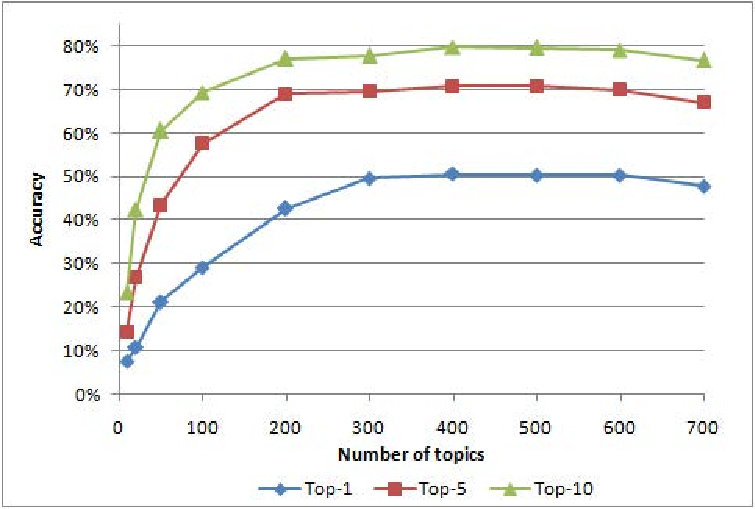
\includegraphics[width=3.3in]{sensitive}
\caption{Top-ranked Accuracy with Different Numbers of Topics for Eclipse}
\label{sensitive}
\end{figure}

%%\begin{figure}
%%\centerline{\epsfxsize=3.3in \epsffile{tradeoff.eps}}
%%\caption{Top-ranked Accuracy with Different Numbers of Sampling Size}
%%\label{tradeoff}
%%\end{figure}

\begin{table}[t]
\centering
\caption{Top-ranked Accuracy with Different Sampling Sizes $r$}
\setlength{\tabcolsep}{2.5pt}
\begin{tabular}{|l||r|r|r|r|r|r|r|r|r|r|r|r|r|}
\hline
   r(\%) & 0 & 1 & 5 & 10 & 20 & 30 & 40 & 50 & 60 & 70 & 80 & 90 & 100\\
\hline
   Top-1 (\%) & 47 & 48 & 48 & 49 & 50 & 51 & 51 & 51 & 51 & 51 & 51 & 52 & 52\\
   Top-5 (\%) & 67 & 67 & 69 & 69 & 70 & 70 & 71 & 71 & 71 & 71 & 72 & 72 & 72\\
   Top-10 (\%) & 75 & 75 & 77 & 79 & 79 & 80 & 80 & 81 & 80 & 81 & 81 & 81 & 81\\
\hline
   Time (s) & 17 & 22 & 38 & 58 & 111 & 146 & 190 & 235 & 280 & 330 & 370 & 406 & 477\\
\hline
\end{tabular}
\label{tradeoff}
\end{table}

In our next experiment, we evaluated the sensitivity of accuracy as
the size $r$ of (Gibbs) sampling set varies for incremental updating
of {\model}'s internal data (Section~\ref{updating-algo}). We fixed
the number of topics $K$ at 500 because we used Eclipse data set for
this experiment. We varied the size of the sample set from 0, 1, 5,
10, 20, ..., 90, and 100\% of the full size of existing data. The case
of 100\% means complete re-training. We measured accuracy and the
updating time for each case. As seen in Table~\ref{tradeoff}, when the
sample size of bug reports used for updating the internal model is
small, time efficiency is gained very much with very little accuracy
reduced. For example, with the selection of 10\% of previous bug
reports for model updating, the updating time is 8.2 times smaller but
top-ranked accuracy reduces only from 2-3\%. This result shows that
our selection strategy for a smaller sample set
(Section~\ref{updating-algo}) for incremental updating is efficient
and quite accurate. If a small sample of previous bug reports is
selected such that all duplicate ones are included, accuracy will not
reduce much.


\subsection{Accuracy Comparison}

\begin{figure}[t]
\centering
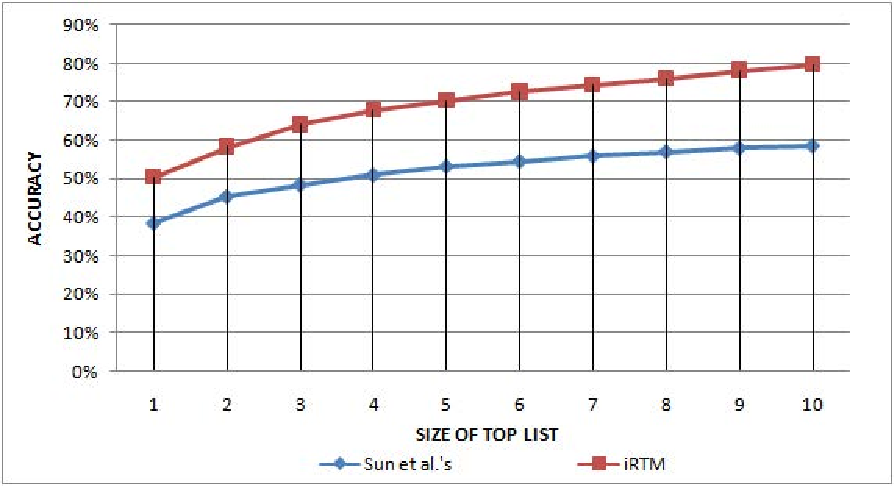
\includegraphics[width=3.3in]{eclipse3}
\caption{Accuracy Comparison with Different Top List Sizes for Eclipse}
\label{eclipse}
\end{figure}


In the next experiment, we compared {\model}'s performance with that
of Sun {\em et al.}'s~\cite{davidlo10}. The parameters of {\model} in
this experiment were selected after fine-tuning for best results as
described earlier. Figure~\ref{eclipse} displays the accuracy result
of {\model} in comparison with Sun {\em et al.}'s on Eclipse data
set. As shown, for a new bug report, {\bf in half of the detection cases,
{\model} can correctly detect the duplication (if any) with just a
single result}. With a list of top 5 resulting bug reports, {\model}
can correctly detect the duplication of a given report in 71\% of the
cases. That is, given a bug report, it can correctly detect its
duplication(s) (if any) within its top-5 recommended bug reports in
almost 3 out of 4 cases. With top lists of 10 reports, it can correctly
detect in 80\% of the cases. In comparison, Sun {\em et al.}'s tool
can achieve the accuracy levels at the top lists of sizes 5 and 10 at
only 53\% and 58\%, respectively. In general, for top lists from 1-10
bug reports, {\bf {\model} achieves higher accuracy than Sun {\em et al.}'s
from 12--22\%}.

\begin{figure}[t]
\centering
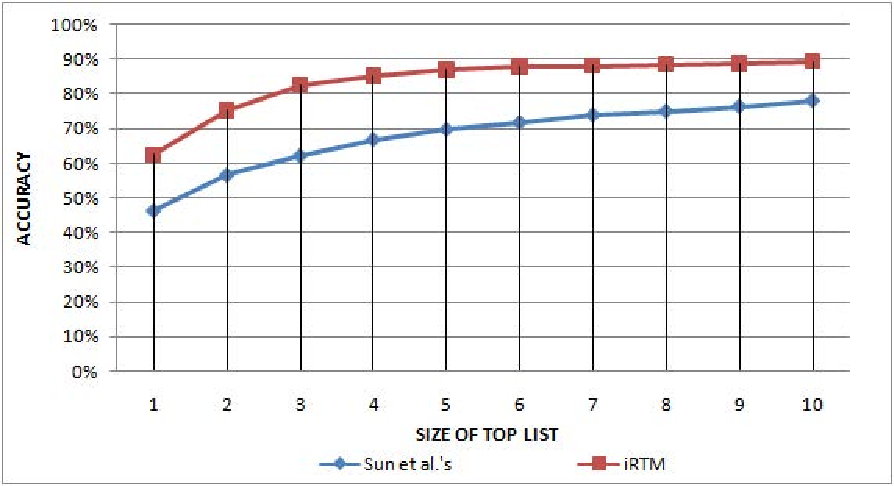
\includegraphics[width=3.3in]{openoffice}
\caption{Accuracy Comparison with Different Top List Sizes for OpenOffice}
\label{openoffice}
\end{figure}

%\begin{figure}[t]
%\centerline{\epsfxsize=3.3in \epsffile{openoffice.eps}}
%\caption{Accuracy Comparison with Different Top List Sizes for OpenOffice}
%\label{openoffice}
%\end{figure}

Figures~\ref{openoffice}, \ref{firefox}, \ref{apache},
\ref{freedesktop}, and \ref{netbeans} display the accuracy results of
    {\model} in comparison with Sun {\em et al.}'s approach on
    OpenOffice, FireFox, Apache, FreeDesktop, and NetBeans datasets,
    respectively. {\bf {\model} consistently achieves very high levels
      of accuracy (with up to 63\% for top-1, 87\% for top-5, and 90\%
      for top-10 accuracy)}. On average for each subject system, the
    top-1, top-5, and top-10 accuracy levels are 56\%, 78\%, and 85\%,
    respectively. For the top-1 to top-10 results, {\bf {\model}
      consistently outperformed Sun {\em et al.}'s with higher
      accuracy from 6--25\%} (from 11--20\% on OpenOffice, 4--9\% on
      FireFox, 6--11\% on Apache, 18--25\% on FreeDesktop, and
      6--11\% on NetBeans datasets).


%%Figure~\ref{openoffice} displays the accuracy result of {\model} in
%%comparison with Sun {\em et al.}'s on OpenOffice data set. As seen,
%%{\model} consistently has very high level of accuracy (63\%, 87\%, and
%%90\% for top-1, top-5, and top-10 accuracy). For the top-1 to top-10
%%results, {\model} achieves higher accuracy than Sun {\em et al.}'s
%%approach from 11\%-20\%.

\begin{figure}[t]
\centering
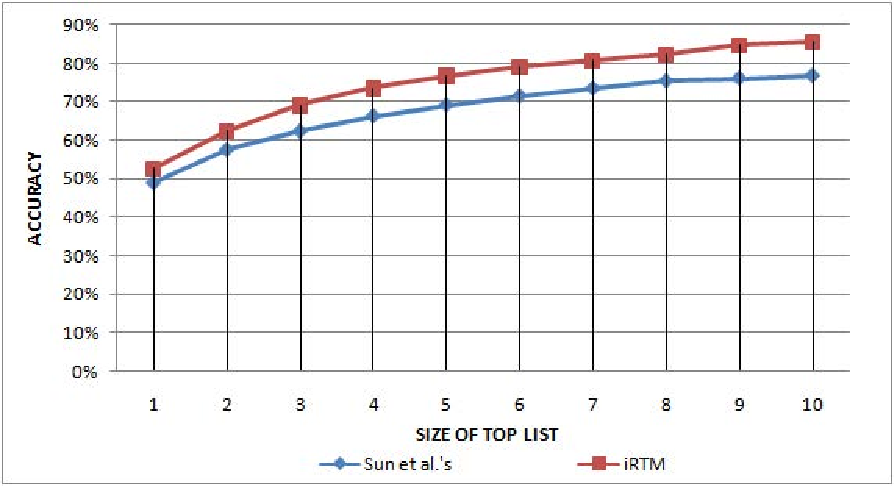
\includegraphics[width=3.3in]{firefox2}
\caption{Accuracy Comparison with Different Top List Sizes for FireFox}
\label{firefox}
\end{figure}

%%Figure~\ref{firefox} displays the accuracy result of {\model} in
%%comparison with Sun {\em et al.}'s on FireFox dataset. As shown,
%%{\model} achieves a higher level of accuracy than their approach. With
%%top lists of 5 and 10 reports, it can correctly determine in 77\% and
%%86\% of the cases, respectively. In comparison, the corresponding
%%numbers at top-5 and top-10 in Sun {\em et al.}'s approach is 70\% and
%%77\%. For the top-1 to top-10 results, {\model} achieves higher
%%accuracy than Sun {\em et al.}'s from 4\%-9\%.

\begin{figure}[t]
\centering
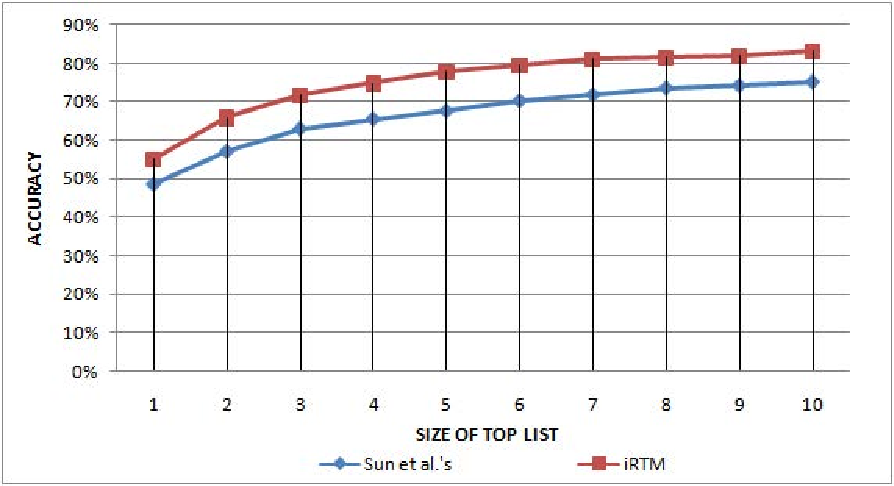
\includegraphics[width=3.3in]{apache}
\caption{Accuracy Comparison with Different Top List Sizes for Apache}
\label{apache}
\end{figure}

%%Figure~\ref{apache} shows {\model}'s accuracy on Apache dataset. As
%%seen, {\model} achieves higher accuracy than Sun {\em et al.}'s
%%from 6\%-11\%. Importantly, it consistently has very high accuracy
%%(78\% and 83\% top-5 and top-10 accuracy).

\begin{figure}[t]
\centering
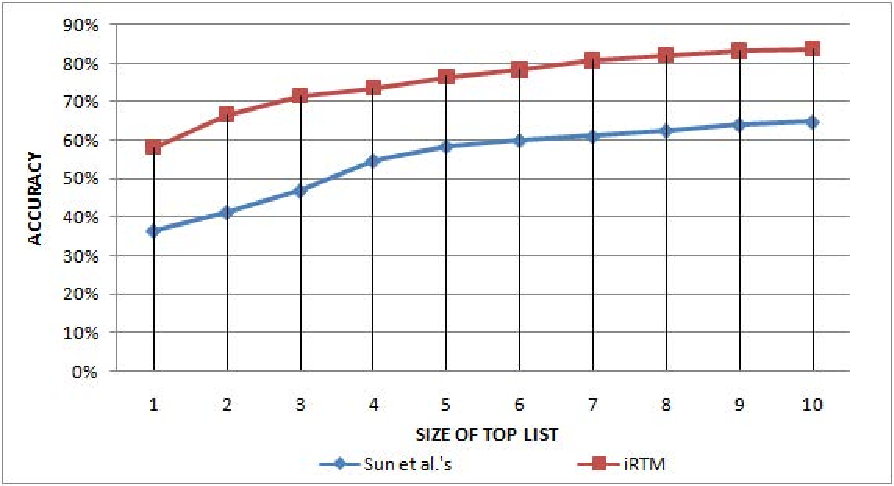
\includegraphics[width=3.3in]{freedesktop}
\caption{Accuracy Comparison with Different Top List Sizes for FreeDesktop}
\label{freedesktop}
\end{figure}

%\begin{figure}[t]
%\centerline{\epsfxsize=3.3in \epsffile{freedesktop.eps}}
%\caption{Accuracy Comparison with Different Top List Sizes for FreeDesktop}
%\label{freedesktop}
%\end{figure}

%%Similarly higher level accuracy was achieved on FreeDesktop dataset
%%for {\model} as shown in Figure~\ref{freedesktop} (77\% top-5 and 84\%
%%top-10 accuracy). For this dataset, {\model} outperformed Sun {\em et
%%al.}'s from 18\%-25\% for top-1 to top-10 lists of results. {\model}
%%also achieves a higher level of accuracy than their approach on the
%%NetBeans dataset (Figure~\ref{netbeans}).

\begin{figure}[t]
\centering
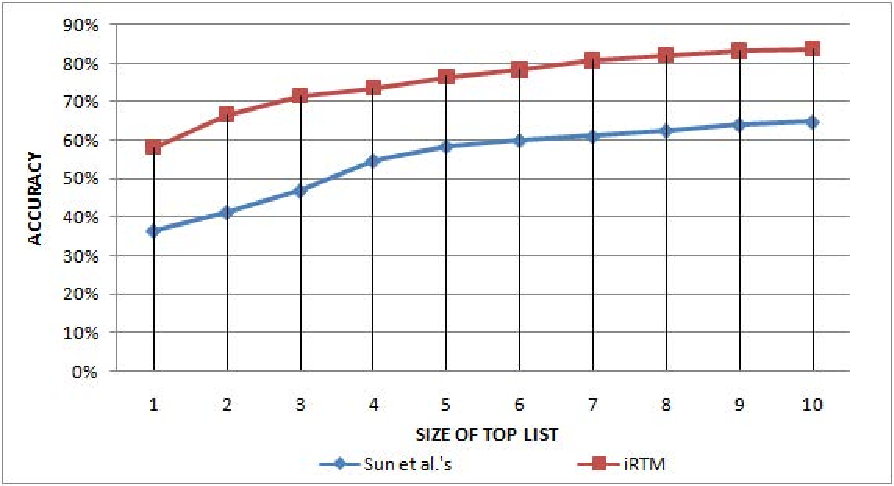
\includegraphics[width=3.3in]{freedesktop}
\caption{Accuracy Comparison with Different Top List Sizes for NetBeans}
\label{netbeans}
\end{figure}

\subsection{Time Efficiency Comparison}

\begin{table*}[t]
\centering
\footnotesize
\caption{Time Efficiency Comparison}
\begin{tabular}{|l||r|r|r|r||r|r|r|r|}
  \hline
     &  & {\model} & & & & Sun's &  & \\
  \hline
  Project & Initial & Average & Update & Prediction & Initial & Average & Re-Training & Prediction \\
          & Training & Update & per Report  & & Training & Re-Training & per Report  & \\
  \hline
  Eclipse & 850s & 150s & 0.25s & 1.7s & 810s & 860s & 1.4s & 25s\\
  OpenOffice & 485s & 65s & 0.09s & 1.4s & 334s & 350s & 0.5s & 18s \\
  FireFox & 1,280s & 182s & 0.09s & 4.3s & 1,350s & 1,420s & 0.7s & 73s\\
  Apache  & 711s & 88.5s & 0.08s & 1.7s & 491s & 522s & 0.53s & 36s \\
  FreeDesktop & 833s & 93.5s & 0.09s & 2.1s & 546s & 576s & 0.58s & 43s\\
  NetBeans & 953s & 181.5s & 0.18s & 2.7s & 972s & 1,024s & 1s & 67s\\
  \hline
\end{tabular}
\label{timetab}
\end{table*}

%\begin{table}[t]
%\centering
%\footnotesize
%\caption{Time Efficiency Comparison}
%\begin{tabular}{|l||r|r|r||r|r|r|}
%  \hline
%     &  & {\model} & & & Sun's &  \\
%  \hline
%  Project & Initial & Update & Pred. & Initial & Re-Train & Pred. \\
%          & Train &  &  & Train &  & \\
%  \hline
%  Eclipse & 850s & 150s & 17s & 810s & 860s & 25s\\
%  FireFox & 1,280s & 182s  & 43s & 1,350s & 1,420s & 73s\\
%  OpenOffice & 485s & 65s & 13.5s & 334s & 350s & 18s \\
%  \hline
%\end{tabular}
%\label{timetab}
%\end{table}

During running two tools on the collected data sets, we also recorded
the execution time. Table~\ref{timetab} displays the result. Column
\code{Initial Training} shows the amount of initial training time of
the corresponding tool for the first data frame. Column \code{Average
Update} displays the average updating time for {\model} for each data
frame. In contrast, Sun {\em et al.}'s needs to re-train the data and
its average re-training time for each frame is in the column
\code{Average Re-Training}. Column \code{Update per Report} shows the
updating time for each bug report for {\model}, while column
\code{Re-training per Report} is for average re-training time per bug
report in Sun {\em et al.}'s. Column \code{Prediction}
shows the corresponding prediction time for each bug report.

{\model} is much more efficient than Sun {\em et al.}'s SVM approach,
especially for large datasets. {\model} took much shorter time (many
times faster) for data updating than complete re-training time in
their approach. On average, for a new bug report, it took only about
0.14s for {\model} to update its data.
%The training time in {\model} is proportional to the number of bug
%reports as we will show it later.
The complete re-training time in Sun {\em et al.}'s is in fact higher
than that of its initial training because in later data frames, more bug
reports were included. That is, the more bug reports come, the higher
its complete re-training time will be.

%For the model updating with 120 new bug reports, it took only 1 hour
%in training for {\model}. For a new bug report, it took only 30
%seconds for duplication detection.

\subsection{Scalability}

In our third experiment, we evaluated the scalability of {\model}
for a large data set. In this experiment, we prepared a larger dataset
of Eclipse's bug reports with a longer history. We chose Eclipse's
platform component  with 61,110 bug
reports, in which 14,020 are determined by Eclipse's developers as
duplicate ones.  The sizes of vocabulary sets is 120,372 terms. 
%(In the previous experiment for comparing {\model} with Sun {\em et
%  al.}'s approach, we did not use this data set because SVM cannot
%scale.)

Figure~\ref{time} shows the dependence between training time and the
number of bug reports in Eclipse's dataset. As shown, the amount of
training time increases almost linearly with respect to the number of
bug reports and their duplicate indicators (We keep the number of
iterations of Gibbs sampling the same). This is a key advantage of
{\model} over the SVM-based model in Sun {\em et al.}~\cite{davidlo10}
where the complete training time increases significantly as the number
of bug reports increases. Importantly, the update time with
incremental training is much smaller than that of the complete
re-training, and {\model} still scales well as the number of bug
reports increases.

\begin{figure}[t]
\centering
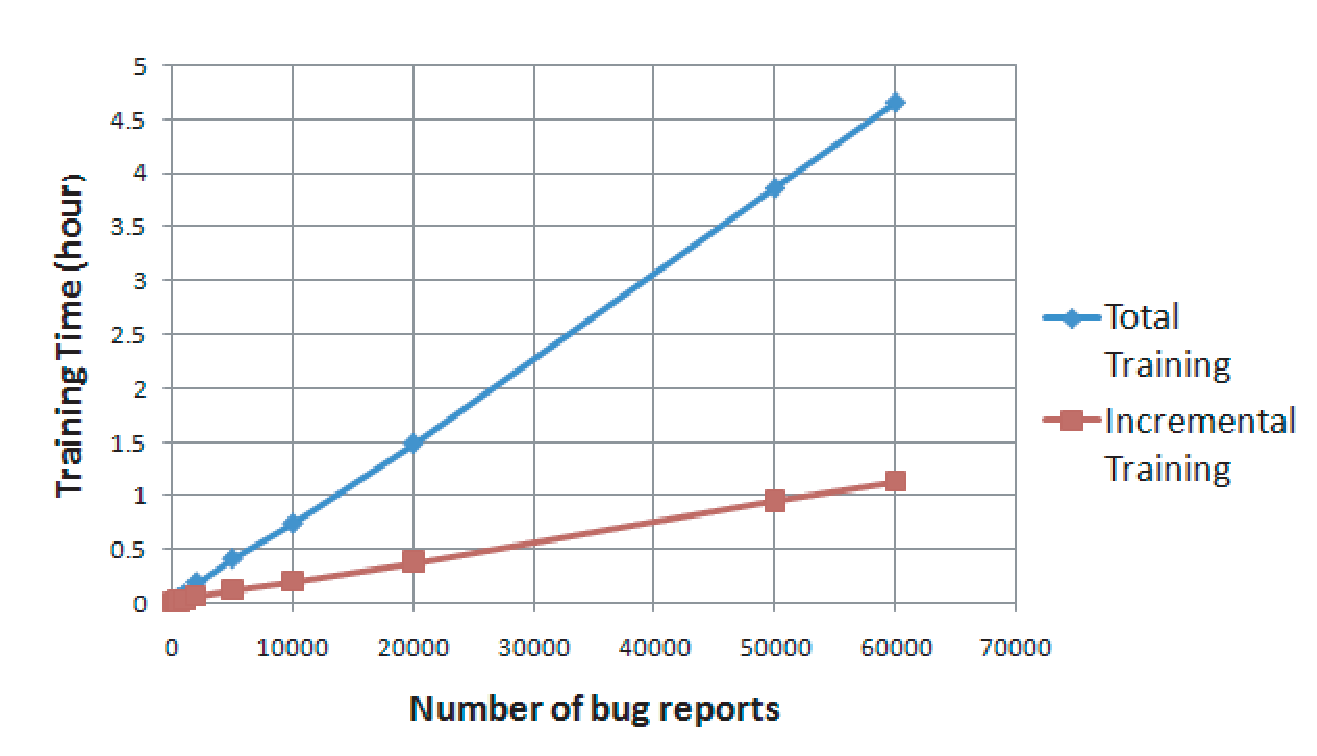
\includegraphics[width=3.5in]{time}
\caption{Training Time for Eclipse's Data}
\label{time}
\end{figure}

%begin{figure}[t]
%centerline{\epsfxsize=3.5in \epsffile{time.eps}}
%caption{Training Time for Eclipse's Data}
%label{time}
%end{figure}

%Importantly, to compare the result from an incremental run with that
%of a fully re-training run, we compared the detection results after 7,
%14, 21, and so on frames between two runs. In all cases, both runs
%gave no significantly different results.

%\subsection{Threats to Validity}

 %\subsection{Interesting Case Studies}

%Let us discuss a few real-world examples that we found during our
%experimental studies.



%Figure {\ref{bugreport225337}} shows two duplicate bug reports
%detected by {\model}. Except the terms NPE
%(\code{NullPointerException}) and \code{StructuredViewer}, which are
%popular and common in the project, the two reports contain several
%different terms because the reporters found the bug in two different
%usage scenarios. That leads to different exception traces: one
%involving image updating, and another on widget selection. We noticed
%that when running BM25F model by itself, bug report \#225169 is ranked
%8$^{th}$ in the list that could be duplicate of bug report \#225337
%due to the dissimilarity in texts. However, after extracting topics
%via the co-occurrences of other terms such as \code{startup},
%\code{first time}, \code{RSE perspective}, \code{wizard}, etc in the
%previous duplicate reports (e.g. from bug report \#218304, not shown),
%{\model} ranked it at the highest position and detected them as
%duplicate ones.

%\begin{figure}
%\vspace{2mm}
%\sf
%\small
%
%\textbf{Bug Report \#225169}\\
%\textbf{Summary}:  Get NPE when startup RSE on a new workspace\\
%\textbf{Description}:\\
%	Using Eclipse M5 driver and RSE I20080401-0935 build. Start
%	eclipse on a new workspace, and switch to RSE perspective. I
%	could see the following error in the log. But
%	otherwise, things are normal.\\ java.lang.NullPointerException
%	at\\
%	org.eclipse.....getImageDescriptor(SystemView...java:123)\\
%	...\\ at
%	org.eclipse....doUpdateItem(AbstractTreeViewer.java:1010)\\ at
%	org.eclipse....doUpdateItem(SafeTreeViewer.java:79)\\ at
%	org.eclipse....run(StructuredViewer.java:466)...\\
%	-----------------------------------------------------------------------\\
%\textbf{Bug Report \#225337}\\
%\textbf{Summary}:  NPE when selecting linux connection in wizard for the first time\\
%\textbf{Description}:\\
%	After starting an eclipse for the first time, when I went select Linux in the
%	new connection wizard, I hit this exception.  When I tried again a few times
%	later, I wasn't able to hit it.\\
%	java.lang.NullPointerException at\\
%	org.eclipse....getAdditionalWizardPages(RSEDefault...:404)\\
%	...\\
%	at org.eclipse....updateSelection(StructuredViewer.java:2062)\\
%	at org.eclipse....handleSelect(StructuredViewer.java:1138)\\
%	at org.eclipse....widgetSelected(StructuredViewer.java:1168)...\\
%\caption{Duplicate Bug Reports in Eclipse}
%\label{bugreport225337}
%\end{figure}

%-------------------------------------------------------------------------
% SECOND EXAMPLE
%-------------------------------------------------------------------------

\begin{figure}[t]
%\scriptsize
%\sf
\small
\textbf{Bug Report \#240790}\\
\textbf{Summary}: [search] callers are not found when caller and callee reside in sibling Java projects\\
\textbf{Description}:\\
	1. create a java project "common" having one interface\\...
	6. Client.init() is not found being a caller (search cope might be
	"Workspace" or "Hierarchy")\\
-----------------------------------------------------------------------\\
\textbf{Bug Report \#250454}\\
\textbf{Summary}:   [search] Cannot find method references between projects\\
\textbf{Description}:\\
	1) define 3 projects: rootProject, subProject1, and subProject2.\\
	2) set project build depedencies such that subProject1 and subProject2 depend
	on rootProject...\\
	6) Search for references to Square.f() directly from it's declaration in
	Square.java.\\
			6a) EXPECT: one result: ShapeUser.useShape(Shape)\\
			6b) ACTUAL: no results\\
	If ShapeUser is instead located in the direct derivable project dependency
	graph for subProject1, the results are ok....\\
			1) If Square were defined in rootProject itself, the search succeeds.\\
			2) If Square were defined in subProject2, the search succeeds. \\
			3) If subProject2 has a build dependency on subProject1, the search
	succeeds.\\

	Additionally, searching for references to f() from the Shape declaration
	succeeds as defined above.  It appears the search does not go to all dependent
	projects of the project declaring the interface....\\
\caption{Duplicate Bug Reports \#250454 and \#240790}
\label{bugreport250454}
\end{figure}

\vspace{0.04in}
\noindent {\bf Interesting Case Studies} An example of detected duplicate bug reports 
is in Figure~\ref{bugreport250454}. The texts in two summaries are
different. The re-producing steps described by two bug reporters are
totally different. As running with the Sun {\em et al.}'s model alone, bug
report \#240790 was ranked 6th in the list of potential duplications
of bug report \#250454. Trained with historical data via identified
duplicate reports of \#250454 (not shown), DBTM can learn sets of
different terms describing the same technical issue in this new
report, which is the issue of searching objects dependent on sibling
projects.

%Final
%More examples are shown on our project's web site.
%(\url{http://home.engineering.iastate.edu/~anhnt/Research/DBTM/})

%, real duplicate group (bug report \#240790) of bug report \#250454 is
%ranked sixth in the ranked list of BM25f model because the two bugs do
%not has much text similarity (they only share important word
%\code{search}).  The duplicate group is ranked first in our experiment
%using DBTM, since the model can learn that the two bug reports
%\#240790 and \#250454) infer to the issue when searching objects on
%dependent (sibling) projects.

%We also find hundreds of cases where DBTM can elevate the ranked of
%real duplicate group in the ranked list of potential duplicate groups
%of a bug report, in comparison with BM25f model. See our website for
%our finding.


\vspace{0.04in}
\noindent {\bf Threats to Validity.}  We evaluated only on six
open-source projects in which three of them are from an existing work
on duplication bug report detection. We cannot ensure {\model} will
work well in other projects where different projects might have
different quality of bug reports.  However, Eclipse, Mozilla and
OpenOffice are long-lasting projects and were used in prior
research. They are sufficiently representative for our comparison. We
also should validate our method on commercial projects.

%
%For comparison, we re-implemented the SVM technique in Sun {\em et
%  al.}~\cite{davidlo10}, rather using their tool (which is not
%available). However, we followed exactly their description in their
%paper~\cite{davidlo10}, and used the same machine learning tool
%LIBSVM~\cite{libsvm} as in their work to re-implement it.


%The training time is a function of number of bug reports, number of
%duplicate links, number of iterations of Gibbs sampling.
%However, through experiment, the value is almost a linear function of
%the number of bug reports and the number of duplicate links.
%When the number of of duplicate links increases, iRTM ensures that the
%training time not increasing explosively.
%The update time when we use the incremental mechanism is even more
%faster. Figure (~\ref{time}) shows the dependence of update time as a
%function of number of samples used for random Gibbs sampling and the
%size of bug reports.



%\begin{figure}[h]
%	\includegraphics[width=3.6in,angle=270]{TrainingTime1.eps}
%	\caption{Training time for Eclipse}
%	\label{fig:TrainingTime1}
%\end{figure}

%Comparing with Sun {\em et al.}'s approach~\cite{davidlo10}, their
%average accuracy levels at the top lists of sizes 5,10, and 20 are
%41\%, 60\%


\section{Related Work}

A related work to {\model} is the Support Vector Machine (SVM)-based
approach from Sun {\em et al.}~\cite{davidlo10}.  In the training
phase of their model, all the pairs of duplicate bug reports are
formed and considered as the positive samples. All other pairs of
non-duplicate bug reports are used as the negative samples. For each
sample (i.e. a pair of reports), a total of 54 features are
extracted. Each feature is represented by the sum of all inverse
values of the frequencies of documents containing terms or bi-grams
(i.e. two consecutive terms) that appear in the summaries and/or
descriptions of both bug reports in the sample. All positive and
negative pairs/samples are used to train and derive the parameters of
a SVM model. In the prediction phase, as a new report arrives, it
would be paired with all existing reports. Then, each pair would be
fed into the trained SVM model and be classified as positive or
negative. Positive pairs imply duplicate reports. Finally, if a new
bug report is predicted by SVM model as duplicate, it is compared
with existing bug reports to determine its master bug report.

There are key advances of {\model} over their SVM model. First, their
model is not suitable for software evolution. It cannot work in an
{\em incremental} manner. For new bug reports, their model requires
complete re-training. As the project evolves, the bug report data gets
increasingly large, the training set continually grows, and the
re-training time will keep increasing significantly. The reason is
that as more reports are added, the numbers of (negative and positive)
pairs/samples will dramatically increase due to the nature of pairing
in the SVM model. With the speed of 3-5 new bug reports per hour
(e.g. in Eclipse)~\cite{davidlo10}, their time cost of for fully
re-training is much higher than {\model}'s updating time.

%not quite practical. In contrast, {\model} can incrementally update
%its parameters in very short time as new data is available.

Another disadvantage of their approach is that, the SVM model predicts
that a new report is a duplication of multiple existing bug reports
but requires a second phase to rank which one is more likely than
others. That is, after predicting the duplication of a new bug report,
their tool performs a second phase to determine the list of potential
master reports. This adds extra computational time. In contrast,
{\model} is able to rank potential master reports based on the
probabilities of generating corresponding pairs of reports. The reason
is that {\model} treats the problem of detecting duplication reports
as a {\em ranking problem}, while their SVM-based approach considers
it as a {\em classification one}. Moreover, in contrast to our
generative model, their model is SVM, a discriminative model. The
quality of their results depends very much on the positive and
negative sets of samples. Because the percentage of duplicate bug
reports is much smaller than that of non-duplicate ones in the
project, the negative set will grow faster and their approach faces
the issue of un-balance between positive and negative samples. With
the generative approach, {\model} does not have to deal with negative
and positive sample sets. Instead, it decides the probability of
generating a pair of duplicate bug reports.

To overcome that, Sun {\em et al.}~\cite{sun-ase11} introduced REP, a
novel IR technique that extends BM25F to consider the long bug reports
and the meta-data such as the reported product, component, and
version. They showed that REP outperformed the state-of-the-art ML
approaches in both accuracy and efficiency. We did not compare with REP
because it is IR-based while we used machine learning.
%XW
%In this work, we combine BM25F with our novel topic model, T-Model, to
%address the cases where duplicate reports have different terms for the
%same technical issue. To our knowledge, DBTM is the first work in
%which topic-based features are used with IR to support the detection
%of duplicate bug reports.
%
Jalbert and Weimer~\cite{weimer08} use a binary classifier model for
predicting duplicate bug reports. They utilizes a linear regression
over {\em textual} features of bug reports computed from the
frequencies of terms in bug reports.
%%%To make a binary classifier, they specify an output value cutoff over
%%%such features that distinguishes between duplicate and non-duplicate
%%%status.
Similar to Sun {\em et al.}'s model, this model requires complete
re-training for new bug reports.
%, which is not quite efficient in practice.
Moreover, their model relies solely on {\em textual similarity}, while
{\model} focuses more on the underlying {\em technical topics} of bug
reports to determine the duplications.
%Finally, their model is discriminative, thus, facing the issue of
%unbalanced positive and negative sample sets of bug reports.

One of the first techniques to detect duplicate bug reports is Runeson
{\em et al.}'s~\cite{runeson07}. In contrast to aforementioned machine
learning (ML) approaches, Runeson {\em et al.}  utilize a natural
language processing (NLP) approach.
%The bug reports are parsed, stemmed, and the stopwords are
%removed.
Each report is modeled by a vector of textual features. The
feature of such a vector at a position corresponding to a term is
computed based on Term frequency-Inverse document
frequency~\cite{salton73}. Vector similarity is used to measure the
similarity among bug reports.
%Given a bug report under investigation, their tool returns similar bug
%reports based on the vector similarities between the new report and
%the existing ones.
Hiew~\cite{hiew06}'s approach for duplicate bug report detection is
based on information retrieval (IR) as in Runeson's. However, it uses
incremental clustering for further grouping of duplicate reports.
%is based on incremental clustering, which is quite similar to
%information retrieval. The main difference is that Hiew�s approach
%further considers the detected duplicate bug-report pairs/groups as
%clusters. Thus, when calculating similarities between a new report
%and existing bug reports, each detected cluster is considered as a
%whole rather than as several individual existing bug reports. That
%is to say, for each detected cluster, this approach will calculate one
%similarity between the new report and the detected cluster instead
%of calculating several similarities between the new report and all
%the reports in the cluster.
Comparing to those approaches, {\model} operates at a higher
abstraction level by comparing the underlying technical topics in
reports, instead of their terms. Moreover, ML approaches have been
shown to outperform NLP/IR approaches~\cite{davidlo10}. Wang {\em et
al.}~\cite{taoxie08} combine NLP with execution trace information in a
report.
%%%They utilize both Tf and Idf for textual feature extraction.
DBTM~\cite{ase12} uses a combination of IR and topic modeling.
We do not use IR in this work, therefore, we did not compare our work
with DBTM.
%Despite performance improvement, their approach is not always
%applicable in the cases where execution information considered in
%their tool is not available.
%%%and hard to collect,
%%%especially for binary programs. Sun {\em et al.}~\cite{davidlo10}
%%%reported that the percentage of reports having execution information
%%%is very low (0.83\%).

Other researchers also focus on bug reports. It is suggested that
duplicate bug reports complement to one another to help
in bug fixing~\cite{bettenburg-icsm-2008}. 
%%Bettenburg {\em et al.}~\cite{rahul08} analyzed information mismatch
%%between what developers need and what users supply to determine good
%%properties in bug reports. 
Structural information from bug reports has been shown to be
useful~\cite{bettenburg-msr08,ko06}.
%%Hooimeijer and Weimer~\cite{weimer-ase07} develop a statistic-based
%%model to automatically predict the quality of bug reports.
%Ko {\em et al.}~\cite{ko06} perform linguistic analysis on bug reports
%and suggest more structure for their contents.
Other researchers categorize bug reports based on types, quality, or
severity~\cite{rahul08,weimer-ase07,anvik06,andy-pod03,cubranic04,menzies08,bettenburg-eclipse07,weimer06,lucca02,fischer03,Sandusky04bugreport}.
%However, none of them addresses the automatic detection of duplicate
%bug reports.
From bug reports, prediction tools~\cite{weiss07,skim06} can tell
whether a bug could be resolved with certain fixing time. Approaches
for automatic assignments of bug fixers include
~\cite{anvik06,Canfora05howsoftware}.
%canfora-sac06}.
%%Other approaches aim to study the relationships among bug
%%reports~\cite{fischer03,Sandusky04bugreport}. 
Gethers and Poshyvanyk~\cite{gethers10} utilize RTM in capturing the
latent topics in classes and their relationships.





%and Whitehead claim that the time it takes to fix a
%bug is a useful software quality measure [8]. They measure
%the time taken to fix bugs in two software projects. We
%predict whether a bug will eventually be resolved as a duplicate
%and are not focused on particular resolution times or
%the total lifetime of real bugs.





\section{Conclusions}

We propose a probabilistic model for detecting duplicate bug
reports. 
%%Each bug report is considered as a textual document about
%%technical aspects of a system. 
Duplicate bug reports are the ones similarly describing the same buggy
technical topics. We adapt RTM to formulate the probabilistic
structures of technical aspects in a collection of bug reports and the
duplication indicators among them.
%Trained with prior data on identified duplicate reports, the model is
%used to detect not-yet-identified duplicate ones. 
We also extend RTM into iRTM in which the trained model can be quickly
updated. Our evaluation on real-world systems shows that iRTM is more
accurate and time efficient than the state-of-the-art approach in Sun
{\em et al.}~\cite{davidlo10}.

%to formulate the probabilistic structures of
%technical topics in the collection of bug reports, and to find the
%indicators of the duplication among them based on those topic
%structures. 

\bibliographystyle{IEEEtran}

\bibliography{icsme18}



%\hfill mds
 
%\hfill August 26, 2015

% An example of a floating figure using the graphicx package.
% Note that \label must occur AFTER (or within) \caption.
% For figures, \caption should occur after the \includegraphics.
% Note that IEEEtran v1.7 and later has special internal code that
% is designed to preserve the operation of \label within \caption
% even when the captionsoff option is in effect. However, because
% of issues like this, it may be the safest practice to put all your
% \label just after \caption rather than within \caption{}.
%
% Reminder: the "draftcls" or "draftclsnofoot", not "draft", class
% option should be used if it is desired that the figures are to be
% displayed while in draft mode.
%
%\begin{figure}[!t]
%\centering
%\includegraphics[width=2.5in]{myfigure}
% where an .eps filename suffix will be assumed under latex, 
% and a .pdf suffix will be assumed for pdflatex; or what has been declared
% via \DeclareGraphicsExtensions.
%\caption{Simulation results for the network.}
%\label{fig_sim}
%\end{figure}

% Note that the IEEE typically puts floats only at the top, even when this
% results in a large percentage of a column being occupied by floats.


% An example of a double column floating figure using two subfigures.
% (The subfig.sty package must be loaded for this to work.)
% The subfigure \label commands are set within each subfloat command,
% and the \label for the overall figure must come after \caption.
% \hfil is used as a separator to get equal spacing.
% Watch out that the combined width of all the subfigures on a 
% line do not exceed the text width or a line break will occur.
%
%\begin{figure*}[!t]
%\centering
%\subfloat[Case I]{\includegraphics[width=2.5in]{box}%
%\label{fig_first_case}}
%\hfil
%\subfloat[Case II]{\includegraphics[width=2.5in]{box}%
%\label{fig_second_case}}
%\caption{Simulation results for the network.}
%\label{fig_sim}
%\end{figure*}
%
% Note that often IEEE papers with subfigures do not employ subfigure
% captions (using the optional argument to \subfloat[]), but instead will
% reference/describe all of them (a), (b), etc., within the main caption.
% Be aware that for subfig.sty to generate the (a), (b), etc., subfigure
% labels, the optional argument to \subfloat must be present. If a
% subcaption is not desired, just leave its contents blank,
% e.g., \subfloat[].


% An example of a floating table. Note that, for IEEE style tables, the
% \caption command should come BEFORE the table and, given that table
% captions serve much like titles, are usually capitalized except for words
% such as a, an, and, as, at, but, by, for, in, nor, of, on, or, the, to
% and up, which are usually not capitalized unless they are the first or
% last word of the caption. Table text will default to \footnotesize as
% the IEEE normally uses this smaller font for tables.
% The \label must come after \caption as always.
%
%\begin{table}[!t]
%% increase table row spacing, adjust to taste
%\renewcommand{\arraystretch}{1.3}
% if using array.sty, it might be a good idea to tweak the value of
% \extrarowheight as needed to properly center the text within the cells
%\caption{An Example of a Table}
%\label{table_example}
%\centering
%% Some packages, such as MDW tools, offer better commands for making tables
%% than the plain LaTeX2e tabular which is used here.
%\begin{tabular}{|c||c|}
%\hline
%One & Two\\
%\hline
%Three & Four\\
%\hline
%\end{tabular}
%\end{table}


% Note that the IEEE does not put floats in the very first column
% - or typically anywhere on the first page for that matter. Also,
% in-text middle ("here") positioning is typically not used, but it
% is allowed and encouraged for Computer Society conferences (but
% not Computer Society journals). Most IEEE journals/conferences use
% top floats exclusively. 
% Note that, LaTeX2e, unlike IEEE journals/conferences, places
% footnotes above bottom floats. This can be corrected via the
% \fnbelowfloat command of the stfloats package.




%\section{Conclusion}
%The conclusion goes here.




% conference papers do not normally have an appendix


% use section* for acknowledgment
%\section*{Acknowledgment}


%The authors would like to thank...





% trigger a \newpage just before the given reference
% number - used to balance the columns on the last page
% adjust value as needed - may need to be readjusted if
% the document is modified later
%\IEEEtriggeratref{8}
% The "triggered" command can be changed if desired:
%\IEEEtriggercmd{\enlargethispage{-5in}}

% references section

% can use a bibliography generated by BibTeX as a .bbl file
% BibTeX documentation can be easily obtained at:
% http://mirror.ctan.org/biblio/bibtex/contrib/doc/
% The IEEEtran BibTeX style support page is at:
% http://www.michaelshell.org/tex/ieeetran/bibtex/
%\bibliographystyle{IEEEtran}
% argument is your BibTeX string definitions and bibliography database(s)
%\bibliography{IEEEabrv,../bib/paper}
%
% <OR> manually copy in the resultant .bbl file
% set second argument of \begin to the number of references
% (used to reserve space for the reference number labels box)
%\begin{thebibliography}{1}

%\bibitem{IEEEhowto:kopka}
%H.~Kopka and P.~W. Daly, \emph{A Guide to \LaTeX}, 3rd~ed.\hskip 1em plus
%  0.5em minus 0.4em\relax Harlow, England: Addison-Wesley, 1999.
%
%\end{thebibliography}




% that's all folks
\end{document}


